% Options for packages loaded elsewhere
\PassOptionsToPackage{unicode}{hyperref}
\PassOptionsToPackage{hyphens}{url}
\PassOptionsToPackage{dvipsnames,svgnames,x11names}{xcolor}
%
\documentclass[
  letterpaper,
  DIV=11,
  numbers=noendperiod]{scrartcl}

\usepackage{amsmath,amssymb}
\usepackage{iftex}
\ifPDFTeX
  \usepackage[T1]{fontenc}
  \usepackage[utf8]{inputenc}
  \usepackage{textcomp} % provide euro and other symbols
\else % if luatex or xetex
  \usepackage{unicode-math}
  \defaultfontfeatures{Scale=MatchLowercase}
  \defaultfontfeatures[\rmfamily]{Ligatures=TeX,Scale=1}
\fi
\usepackage{lmodern}
\ifPDFTeX\else  
    % xetex/luatex font selection
\fi
% Use upquote if available, for straight quotes in verbatim environments
\IfFileExists{upquote.sty}{\usepackage{upquote}}{}
\IfFileExists{microtype.sty}{% use microtype if available
  \usepackage[]{microtype}
  \UseMicrotypeSet[protrusion]{basicmath} % disable protrusion for tt fonts
}{}
\makeatletter
\@ifundefined{KOMAClassName}{% if non-KOMA class
  \IfFileExists{parskip.sty}{%
    \usepackage{parskip}
  }{% else
    \setlength{\parindent}{0pt}
    \setlength{\parskip}{6pt plus 2pt minus 1pt}}
}{% if KOMA class
  \KOMAoptions{parskip=half}}
\makeatother
\usepackage{xcolor}
\setlength{\emergencystretch}{3em} % prevent overfull lines
\setcounter{secnumdepth}{5}
% Make \paragraph and \subparagraph free-standing
\ifx\paragraph\undefined\else
  \let\oldparagraph\paragraph
  \renewcommand{\paragraph}[1]{\oldparagraph{#1}\mbox{}}
\fi
\ifx\subparagraph\undefined\else
  \let\oldsubparagraph\subparagraph
  \renewcommand{\subparagraph}[1]{\oldsubparagraph{#1}\mbox{}}
\fi

\usepackage{color}
\usepackage{fancyvrb}
\newcommand{\VerbBar}{|}
\newcommand{\VERB}{\Verb[commandchars=\\\{\}]}
\DefineVerbatimEnvironment{Highlighting}{Verbatim}{commandchars=\\\{\}}
% Add ',fontsize=\small' for more characters per line
\usepackage{framed}
\definecolor{shadecolor}{RGB}{241,243,245}
\newenvironment{Shaded}{\begin{snugshade}}{\end{snugshade}}
\newcommand{\AlertTok}[1]{\textcolor[rgb]{0.68,0.00,0.00}{#1}}
\newcommand{\AnnotationTok}[1]{\textcolor[rgb]{0.37,0.37,0.37}{#1}}
\newcommand{\AttributeTok}[1]{\textcolor[rgb]{0.40,0.45,0.13}{#1}}
\newcommand{\BaseNTok}[1]{\textcolor[rgb]{0.68,0.00,0.00}{#1}}
\newcommand{\BuiltInTok}[1]{\textcolor[rgb]{0.00,0.23,0.31}{#1}}
\newcommand{\CharTok}[1]{\textcolor[rgb]{0.13,0.47,0.30}{#1}}
\newcommand{\CommentTok}[1]{\textcolor[rgb]{0.37,0.37,0.37}{#1}}
\newcommand{\CommentVarTok}[1]{\textcolor[rgb]{0.37,0.37,0.37}{\textit{#1}}}
\newcommand{\ConstantTok}[1]{\textcolor[rgb]{0.56,0.35,0.01}{#1}}
\newcommand{\ControlFlowTok}[1]{\textcolor[rgb]{0.00,0.23,0.31}{#1}}
\newcommand{\DataTypeTok}[1]{\textcolor[rgb]{0.68,0.00,0.00}{#1}}
\newcommand{\DecValTok}[1]{\textcolor[rgb]{0.68,0.00,0.00}{#1}}
\newcommand{\DocumentationTok}[1]{\textcolor[rgb]{0.37,0.37,0.37}{\textit{#1}}}
\newcommand{\ErrorTok}[1]{\textcolor[rgb]{0.68,0.00,0.00}{#1}}
\newcommand{\ExtensionTok}[1]{\textcolor[rgb]{0.00,0.23,0.31}{#1}}
\newcommand{\FloatTok}[1]{\textcolor[rgb]{0.68,0.00,0.00}{#1}}
\newcommand{\FunctionTok}[1]{\textcolor[rgb]{0.28,0.35,0.67}{#1}}
\newcommand{\ImportTok}[1]{\textcolor[rgb]{0.00,0.46,0.62}{#1}}
\newcommand{\InformationTok}[1]{\textcolor[rgb]{0.37,0.37,0.37}{#1}}
\newcommand{\KeywordTok}[1]{\textcolor[rgb]{0.00,0.23,0.31}{#1}}
\newcommand{\NormalTok}[1]{\textcolor[rgb]{0.00,0.23,0.31}{#1}}
\newcommand{\OperatorTok}[1]{\textcolor[rgb]{0.37,0.37,0.37}{#1}}
\newcommand{\OtherTok}[1]{\textcolor[rgb]{0.00,0.23,0.31}{#1}}
\newcommand{\PreprocessorTok}[1]{\textcolor[rgb]{0.68,0.00,0.00}{#1}}
\newcommand{\RegionMarkerTok}[1]{\textcolor[rgb]{0.00,0.23,0.31}{#1}}
\newcommand{\SpecialCharTok}[1]{\textcolor[rgb]{0.37,0.37,0.37}{#1}}
\newcommand{\SpecialStringTok}[1]{\textcolor[rgb]{0.13,0.47,0.30}{#1}}
\newcommand{\StringTok}[1]{\textcolor[rgb]{0.13,0.47,0.30}{#1}}
\newcommand{\VariableTok}[1]{\textcolor[rgb]{0.07,0.07,0.07}{#1}}
\newcommand{\VerbatimStringTok}[1]{\textcolor[rgb]{0.13,0.47,0.30}{#1}}
\newcommand{\WarningTok}[1]{\textcolor[rgb]{0.37,0.37,0.37}{\textit{#1}}}

\providecommand{\tightlist}{%
  \setlength{\itemsep}{0pt}\setlength{\parskip}{0pt}}\usepackage{longtable,booktabs,array}
\usepackage{calc} % for calculating minipage widths
% Correct order of tables after \paragraph or \subparagraph
\usepackage{etoolbox}
\makeatletter
\patchcmd\longtable{\par}{\if@noskipsec\mbox{}\fi\par}{}{}
\makeatother
% Allow footnotes in longtable head/foot
\IfFileExists{footnotehyper.sty}{\usepackage{footnotehyper}}{\usepackage{footnote}}
\makesavenoteenv{longtable}
\usepackage{graphicx}
\makeatletter
\def\maxwidth{\ifdim\Gin@nat@width>\linewidth\linewidth\else\Gin@nat@width\fi}
\def\maxheight{\ifdim\Gin@nat@height>\textheight\textheight\else\Gin@nat@height\fi}
\makeatother
% Scale images if necessary, so that they will not overflow the page
% margins by default, and it is still possible to overwrite the defaults
% using explicit options in \includegraphics[width, height, ...]{}
\setkeys{Gin}{width=\maxwidth,height=\maxheight,keepaspectratio}
% Set default figure placement to htbp
\makeatletter
\def\fps@figure{htbp}
\makeatother

% load packages
\usepackage{geometry}
\usepackage{xcolor}
\usepackage{eso-pic}
\usepackage{fancyhdr}
\usepackage{sectsty}
\usepackage{fontspec}
\usepackage{titlesec}

%% Set page size with a wider right margin
\geometry{a4paper, total={170mm,257mm}, left=20mm, top=20mm, bottom=20mm, right=50mm}

%% Let's define some colours
\definecolor{uniblue}{HTML}{003865}
\definecolor{burgundy}{HTML}{7D2239}
\definecolor{cobalt}{HTML}{005C8A}
\definecolor{lavender}{HTML}{5B4D94}
\definecolor{leaf}{HTML}{006630}
\definecolor{moss}{HTML}{385A4F}
\definecolor{pillarbox}{HTML}{B30C00}
\definecolor{rust}{HTML}{9A3A06}
\definecolor{sandstone}{HTML}{52473B}
\definecolor{skyblue}{HTML}{005398}
\definecolor{slate}{HTML}{4F5961}
\definecolor{thistle}{HTML}{951272}

%\definecolor{light}{HTML}{E6E6FA} % original from template - redefined below as uni blue at 10 percent:
\colorlet{light}{uniblue!10}
%\definecolor{highlight}{HTML}{800080} % original from template - redefined below as uni's skyblue:
\colorlet{highlight}{skyblue}
%\definecolor{dark}{HTML}{330033} % original from template - redefined below as uni blue at 100 percent:
\colorlet{dark}{uniblue}

%% Let's add the border on the right hand side 
\AddToShipoutPicture{% 
    \AtPageLowerLeft{% 
        \put(\LenToUnit{\dimexpr\paperwidth-3cm},0){% 
            \color{light}\rule{3cm}{\LenToUnit\paperheight}%
          }%
     }%
     % logo
    \AtPageLowerLeft{% start the bar at the bottom right of the page
        \put(\LenToUnit{\dimexpr\paperwidth-2.25cm},27.2cm){% move it to the top right
            \color{light}
\includegraphics[width=2.25cm]{_extensions/nrennie/PrettyPDF/uni_logo_boxed.jpg}
          }%
     }%
}

%% Style the page number
\fancypagestyle{mystyle}{
  \fancyhf{}
  \renewcommand\headrulewidth{0pt}
  \fancyfoot[R]{\thepage}
  \fancyfootoffset{3.5cm}
}
\setlength{\footskip}{20pt}

%% style the chapter/section fonts
\chapterfont{\color{uniblue}\fontsize{20}{16.8}\selectfont}
\sectionfont{\color{uniblue}\fontsize{20}{16.8}\selectfont}
\subsectionfont{\color{skyblue}\fontsize{14}{16.8}\selectfont}
\titleformat{\subsection}
  {\color{uniblue!90}\sffamily\Large\bfseries}{\thesubsection}{1em}{}[{\titlerule[0.8pt]}]
\subsubsectionfont{\color{cobalt}}

\renewcommand\thesection{\color{slate}\arabic{section}}
  
% left align title
\makeatletter
\renewcommand{\maketitle}{\bgroup\setlength{\parindent}{0pt}
\begin{flushleft}
  {\color{uniblue}\sffamily\huge\textbf{\@title}} \vspace{0.3cm} \newline
  {\Large {\@subtitle}} \newline
  \@author
\end{flushleft}\egroup
}
\makeatother

%% Use some custom fonts
\setsansfont{Ubuntu}[
    Path=_extensions/nrennie/PrettyPDF/Ubuntu/,
    Scale=0.9,
    Extension = .ttf,
    UprightFont=*-Regular,
    BoldFont=*-Bold,
    ItalicFont=*-Italic,
    ]

\setmainfont{Ubuntu}[
    Path=_extensions/nrennie/PrettyPDF/Ubuntu/,
    Scale=0.9,
    Extension = .ttf,
    UprightFont=*-Regular,
    BoldFont=*-Bold,
    ItalicFont=*-Italic,
    ]
\KOMAoption{captions}{tableheading}
\makeatletter
\@ifpackageloaded{tcolorbox}{}{\usepackage[skins,breakable]{tcolorbox}}
\@ifpackageloaded{fontawesome5}{}{\usepackage{fontawesome5}}
\definecolor{quarto-callout-color}{HTML}{909090}
\definecolor{quarto-callout-note-color}{HTML}{0758E5}
\definecolor{quarto-callout-important-color}{HTML}{CC1914}
\definecolor{quarto-callout-warning-color}{HTML}{EB9113}
\definecolor{quarto-callout-tip-color}{HTML}{00A047}
\definecolor{quarto-callout-caution-color}{HTML}{FC5300}
\definecolor{quarto-callout-color-frame}{HTML}{acacac}
\definecolor{quarto-callout-note-color-frame}{HTML}{4582ec}
\definecolor{quarto-callout-important-color-frame}{HTML}{d9534f}
\definecolor{quarto-callout-warning-color-frame}{HTML}{f0ad4e}
\definecolor{quarto-callout-tip-color-frame}{HTML}{02b875}
\definecolor{quarto-callout-caution-color-frame}{HTML}{fd7e14}
\makeatother
\makeatletter
\@ifpackageloaded{caption}{}{\usepackage{caption}}
\AtBeginDocument{%
\ifdefined\contentsname
  \renewcommand*\contentsname{Table of contents}
\else
  \newcommand\contentsname{Table of contents}
\fi
\ifdefined\listfigurename
  \renewcommand*\listfigurename{List of Figures}
\else
  \newcommand\listfigurename{List of Figures}
\fi
\ifdefined\listtablename
  \renewcommand*\listtablename{List of Tables}
\else
  \newcommand\listtablename{List of Tables}
\fi
\ifdefined\figurename
  \renewcommand*\figurename{Figure}
\else
  \newcommand\figurename{Figure}
\fi
\ifdefined\tablename
  \renewcommand*\tablename{Table}
\else
  \newcommand\tablename{Table}
\fi
}
\@ifpackageloaded{float}{}{\usepackage{float}}
\floatstyle{ruled}
\@ifundefined{c@chapter}{\newfloat{codelisting}{h}{lop}}{\newfloat{codelisting}{h}{lop}[chapter]}
\floatname{codelisting}{Listing}
\newcommand*\listoflistings{\listof{codelisting}{List of Listings}}
\makeatother
\makeatletter
\makeatother
\makeatletter
\@ifpackageloaded{caption}{}{\usepackage{caption}}
\@ifpackageloaded{subcaption}{}{\usepackage{subcaption}}
\makeatother
\makeatletter
\@ifpackageloaded{tcolorbox}{}{\usepackage[skins,breakable]{tcolorbox}}
\makeatother
\makeatletter
\@ifundefined{shadecolor}{\definecolor{shadecolor}{rgb}{.97, .97, .97}}{}
\makeatother
\makeatletter
\@ifundefined{codebgcolor}{\definecolor{codebgcolor}{named}{light}}{}
\makeatother
\makeatletter
\ifdefined\Shaded\renewenvironment{Shaded}{\begin{tcolorbox}[enhanced, colback={codebgcolor}, sharp corners, boxrule=0pt, frame hidden, breakable]}{\end{tcolorbox}}\fi
\makeatother
\ifLuaTeX
  \usepackage{selnolig}  % disable illegal ligatures
\fi
\usepackage{bookmark}

\IfFileExists{xurl.sty}{\usepackage{xurl}}{} % add URL line breaks if available
\urlstyle{same} % disable monospaced font for URLs
\hypersetup{
  pdftitle={Regression modelling part 1},
  colorlinks=true,
  linkcolor={highlight},
  filecolor={Maroon},
  citecolor={Blue},
  urlcolor={highlight},
  pdfcreator={LaTeX via pandoc}}

\title{Regression modelling part 1}
\author{}
\date{}

\begin{document}
\maketitle

\pagestyle{mystyle}

\renewcommand*\contentsname{Contents}
{
\hypersetup{linkcolor=}
\setcounter{tocdepth}{3}
\tableofcontents
}
\section{Introduction}\label{introduction}

Now that we are comfortable with visualising and manipulating data in R,
we can now proceed onto modelling data. The key idea behind modelling
data is to infer the relationship between an:

\begin{itemize}
\tightlist
\item
  \textbf{outcome (or response) variable} \(y\) and
\item
  an \textbf{explanatory (or predictor) variable} \(x\), which can also
  be referred to as an \textbf{independent variable} or
  \textbf{covariate}.
\end{itemize}

Modelling can be used for two purposes:

\begin{enumerate}
\def\labelenumi{\arabic{enumi}.}
\item
  \textbf{Explanation}: For describing the relationship between an
  outcome variable \(y\) and an explanatory variable \emph{x}, and
  determining the potential significance of such relationships using
  quantifiable measures.
\item
  \textbf{Prediction}: for predicting the outcome variable \(y\) given
  information from one or more explanatory variables.
\end{enumerate}

There are many different modelling techniques. However, we will begin
with one of the easier to understand and commonly-used approaches,
\textbf{linear regression}. In particular, we will start by looking at
\textbf{simple linear regression}, where we only have one explanatory
variable.

\textbf{Note}: Additional information and examples can be found in
\href{https://moderndive.com/5-regression.html}{Chapter 5} of
\href{https://moderndive.com/index.html}{An Introduction to Statistical
and Data Science via R}.

You can download today's session R script below:

\begin{tcolorbox}[enhanced jigsaw, leftrule=.75mm, opacityback=0, colbacktitle=quarto-callout-note-color!10!white, left=2mm, rightrule=.15mm, colframe=quarto-callout-note-color-frame, colback=white, coltitle=black, breakable, bottomtitle=1mm, title=\textcolor{quarto-callout-note-color}{\faInfo}\hspace{0.5em}{Note}, toprule=.15mm, titlerule=0mm, toptitle=1mm, bottomrule=.15mm, opacitybacktitle=0.6, arc=.35mm]

I recommend opening a new Quarto file and using it to create your own
notes as you work through today's exercises. This will help you practice
coding in a structured way, reinforce your learning, and keep a reusable
record of your progress.

\end{tcolorbox}

\section{Simple linear regression}\label{simple-linear-regression}

For a response variable \(y\) and an explanatory variable \(x\), the
data can be expressed as:

\[(y_i, x_i), ~~~~ i = 1,\ldots,n.\] That is, we have \(n\) observations
of \(y\) and \(x\). A statistical model is a mathematical statement
describing the variability in a random variable \(y\), which includes
any relationship with the explanatory variable \(x\). The inclusion of
random (unpredictable) components \(\epsilon\), makes the model
statistical, rather than deterministic. A simple linear regression model
involves, as the name suggests, fitting a linear regression line to the
data. Hence, a simple linear regression model can be written as follows:

\[y_i = \alpha + \beta x_i + \epsilon_i, ~~~~ \epsilon_i \sim N(0, \sigma^2),\]
where

\begin{itemize}
\tightlist
\item
  \(y_i\) is the \(i^{th}\) observation of the response variable;
\item
  \(\alpha\) is the \textbf{intercept} of the regression line;
\item
  \(\beta\) is the \textbf{slope} of the regression line;
\item
  \(x_i\) is the \(i^{th}\) observation of the explanatory variable; and
\item
  \(\epsilon_i\) is the \(i^{th}\) random component.
\end{itemize}

The random components, \(\epsilon_i\), are normally distributed with
mean zero and constant variance \(\sigma^2\), such that we are
essentially adding random white noise to the deterministic part of the
model (\(\alpha + \beta x_i\)). Thus, the full probability model for
\(y_i\) given \(x_i\) (\(y_i | x_i\)) can be written as

\[y_i | x_i \sim N(\alpha + \beta x_i, \sigma^2).\]

Hence, the mean comes from the deterministic part of the model, while
the variance comes from the random part. We shall now look into fitting
a simple linear regression model to some data.

\section{Simple linear regression with one numerical explanatory
variable}\label{simple-linear-regression-with-one-numerical-explanatory-variable}

First, we need to load the following packages into R:

\begin{Shaded}
\begin{Highlighting}[]
\FunctionTok{library}\NormalTok{(tidyverse)    }\CommentTok{\# Data wrangling }
\FunctionTok{library}\NormalTok{(ggplot2)      }\CommentTok{\# Data visualization}
\FunctionTok{library}\NormalTok{(performance)  }\CommentTok{\# Model assessment}
\FunctionTok{library}\NormalTok{(skimr)        }\CommentTok{\# Exploratory analysis}
\FunctionTok{library}\NormalTok{(sjPlot)       }\CommentTok{\# Plot and tables for linear models}
\end{Highlighting}
\end{Shaded}

Student feedback in higher education is extremely important when it
comes to the evaluation of teaching techniques, materials, and
improvements in teaching methods and technologies. However, there have
been studies into potential bias factors when feedback is provided, such
as the physical appearance of the teacher; see
\href{https://www.journals.elsevier.com/economics-of-education-review/}{Economics
of Education Review} for details. Here, we shall look at a study from
student evaluations of \(n=463\) professors from The University of Texas
at Austin. In particular, we will examine the evaluation scores of the
instructors based purely on one numerical variable: their \emph{beauty
score}. Therefore, our simple linear regression model will consist of:

\begin{itemize}
\tightlist
\item
  the numerical outcome variable \emph{teaching score} (\(y\)); and
\item
  the numerical explanatory variable \emph{beauty score} (\(x\)).
\end{itemize}

\subsection{Exploratory data analysis}\label{exploratory-data-analysis}

Before you ever do any statistical modelling of data, you should always
perform an \textbf{exploratory data analysis} of the data. Performing an
exploratory data analysis can give us an idea of the distribution of the
data, and whether it contains any strange values, such as
\textbf{outliers} or \textbf{missing values}. However, more importantly,
it is used to inform which statistical model we should fit to the data.
An exploratory data analysis may involve:

\begin{enumerate}
\def\labelenumi{\arabic{enumi}.}
\tightlist
\item
  Looking at the raw values of the data, either by looking at the
  spreadsheet directly, or using R.
\item
  By computing various summary statistics, such as the \emph{five-number
  summary}, means, and standard deviations.
\item
  Plotting the data using various data visualisation techniques.
\end{enumerate}

Let's examine the data \texttt{evals}. First we read the data (stored in
\texttt{.csv} format) and then we can look at the raw values from
\texttt{evals} using the RStudio pop-up spreadsheet viewer using:

\begin{Shaded}
\begin{Highlighting}[]
\NormalTok{evals }\OtherTok{\textless{}{-}} \FunctionTok{read.csv}\NormalTok{(}\StringTok{"evals.csv"}\NormalTok{)}
\FunctionTok{View}\NormalTok{(evals)}
\end{Highlighting}
\end{Shaded}

At the moment we are only really interested in the instructors teaching
(\texttt{score}) and beauty (\texttt{bty\_avg}) scores, and so we can
look at a subset of the data as follows:

\begin{Shaded}
\begin{Highlighting}[]
\NormalTok{evals.scores }\OtherTok{\textless{}{-}}\NormalTok{ evals }\SpecialCharTok{\%\textgreater{}\%}
\NormalTok{  dplyr}\SpecialCharTok{::}\FunctionTok{select}\NormalTok{(score, bty\_avg)}
\end{Highlighting}
\end{Shaded}

The outcome variable \texttt{score} is a numerical average of the
average teaching score based on students' evaluations between 1 and 5.
The explanatory variable \texttt{bty\_avg} is the numerical variable of
the average \emph{beauty} score from a panel of six students' scores
between 1 and 10. As both variables are numerical, we can compute
summary statistics for them using the \texttt{skim} function from the
\texttt{skimr} package as follows:

\begin{Shaded}
\begin{Highlighting}[]
\NormalTok{evals.scores }\SpecialCharTok{\%\textgreater{}\%}
  \FunctionTok{skim}\NormalTok{()}
\end{Highlighting}
\end{Shaded}

\begin{longtable}[]{@{}ll@{}}
\caption{Data summary}\tabularnewline
\toprule\noalign{}
\endfirsthead
\endhead
\bottomrule\noalign{}
\endlastfoot
Name & Piped data \\
Number of rows & 463 \\
Number of columns & 2 \\
\_\_\_\_\_\_\_\_\_\_\_\_\_\_\_\_\_\_\_\_\_\_\_ & \\
Column type frequency: & \\
numeric & 2 \\
\_\_\_\_\_\_\_\_\_\_\_\_\_\_\_\_\_\_\_\_\_\_\_\_ & \\
Group variables & None \\
\end{longtable}

\textbf{Variable type: numeric}

\begin{longtable}[]{@{}
  >{\raggedright\arraybackslash}p{(\columnwidth - 20\tabcolsep) * \real{0.1795}}
  >{\raggedleft\arraybackslash}p{(\columnwidth - 20\tabcolsep) * \real{0.1282}}
  >{\raggedleft\arraybackslash}p{(\columnwidth - 20\tabcolsep) * \real{0.1795}}
  >{\raggedleft\arraybackslash}p{(\columnwidth - 20\tabcolsep) * \real{0.0641}}
  >{\raggedleft\arraybackslash}p{(\columnwidth - 20\tabcolsep) * \real{0.0641}}
  >{\raggedleft\arraybackslash}p{(\columnwidth - 20\tabcolsep) * \real{0.0641}}
  >{\raggedleft\arraybackslash}p{(\columnwidth - 20\tabcolsep) * \real{0.0641}}
  >{\raggedleft\arraybackslash}p{(\columnwidth - 20\tabcolsep) * \real{0.0641}}
  >{\raggedleft\arraybackslash}p{(\columnwidth - 20\tabcolsep) * \real{0.0513}}
  >{\raggedleft\arraybackslash}p{(\columnwidth - 20\tabcolsep) * \real{0.0641}}
  >{\raggedright\arraybackslash}p{(\columnwidth - 20\tabcolsep) * \real{0.0769}}@{}}
\toprule\noalign{}
\begin{minipage}[b]{\linewidth}\raggedright
skim\_variable
\end{minipage} & \begin{minipage}[b]{\linewidth}\raggedleft
n\_missing
\end{minipage} & \begin{minipage}[b]{\linewidth}\raggedleft
complete\_rate
\end{minipage} & \begin{minipage}[b]{\linewidth}\raggedleft
mean
\end{minipage} & \begin{minipage}[b]{\linewidth}\raggedleft
sd
\end{minipage} & \begin{minipage}[b]{\linewidth}\raggedleft
p0
\end{minipage} & \begin{minipage}[b]{\linewidth}\raggedleft
p25
\end{minipage} & \begin{minipage}[b]{\linewidth}\raggedleft
p50
\end{minipage} & \begin{minipage}[b]{\linewidth}\raggedleft
p75
\end{minipage} & \begin{minipage}[b]{\linewidth}\raggedleft
p100
\end{minipage} & \begin{minipage}[b]{\linewidth}\raggedright
hist
\end{minipage} \\
\midrule\noalign{}
\endhead
\bottomrule\noalign{}
\endlastfoot
score & 0 & 1 & 4.17 & 0.54 & 2.30 & 3.80 & 4.30 & 4.6 & 5.00 & ▁▁▅▇▇ \\
bty\_avg & 0 & 1 & 4.42 & 1.53 & 1.67 & 3.17 & 4.33 & 5.5 & 8.17 &
▃▇▇▃▂ \\
\end{longtable}

This provides us with the following information:

\begin{itemize}
\tightlist
\item
  \texttt{missing}: the number of missing values.
\item
  \texttt{complete}: the number of non-missing values.
\item
  \texttt{n}: the total number of observations.
\item
  \texttt{mean}: the mean or average.
\item
  \texttt{sd}: the standard deviation.
\item
  \texttt{p0}: the \(0^{th}\) percentile: the value at which 0\% of
  values are smaller than it (i.e.~the \emph{minimum}).
\item
  \texttt{p25}: the \(25^{th}\) percentile: the value at which 25\% of
  values are smaller than it (i.e.~the \emph{1st quartile}).
\item
  \texttt{p50}: the \(50^{th}\) percentile: the value at which 50\% of
  values are smaller than it (i.e.~the \emph{median}).
\item
  \texttt{p75}: the \(75^{th}\) percentile: the value at which 75\% of
  values are smaller than it (i.e.~the \emph{3rd quartile}).
\item
  \texttt{p100}: the \(100^{th}\) percentile: the value at which 100\%
  of values are smaller than it (i.e.~the \emph{maximum}).
\item
  \texttt{hist}: provides a snapshot of a histogram of the variable.
\end{itemize}

These summary statistics give us an idea of how both variables are
distributed. For example, the mean teaching score (\texttt{score}) is
4.17 out 5, while the mean beauty score (\texttt{bty\_avg}) is 4.42 out
of 10. Also, the middle 50\% of the data for \texttt{score} lies between
3.8 and 4.6, while the middle 50\% of \texttt{bty\_avg} lies between
3.17 and 5.5.

\subsection{Correlation}\label{correlation}

The above summary statistics provide information about each variable
separately. However, we are interested in a potential relationship
between the two variables and as such it would be of interest to
evaluate some statistic that considers both variables simultaneously.
One such statistic is the \textbf{correlation}, which ranges between -1
and 1 and describes the strength of the linear relationship between two
numerical variables, such that

\begin{itemize}
\tightlist
\item
  -1 indicates a perfect \emph{negative relationship}. That is, as the
  values of one variable increase, the values of the other decrease.
\item
  0 indicates no relationship. The values of both variables
  increase/decrease independently of one another.
\item
  1 indicates a perfect \emph{positive relationship}. That is, the
  values of both variables increase simultaneously.
\end{itemize}

The correlation coefficient \(\rho(\cdot)\) between two variables \(x\)
and \(y\) can be computed as:

\[
\rho (x,y) = \dfrac{\sum_{i=1}^n (x_i -\bar{x})(y_i-\bar{y})}{\sqrt{\sum_{i=1}^n (x_i-\bar{x})^2}\sqrt{\sum_{i=1}^n (y_i-\bar{y})^2}}
\]

Here, \(\bar{x}\) and \(\bar{y}\) denotes the mean of \(x_i\) and
\(y_i\) respectively across \(i= 1,\ldots,n\) observations.The plot
below displays scatterplots for hypothetical numerical variables \(x\)
and \(y\) simulated to have different levels of correlation.

\begin{figure}[H]

{\centering 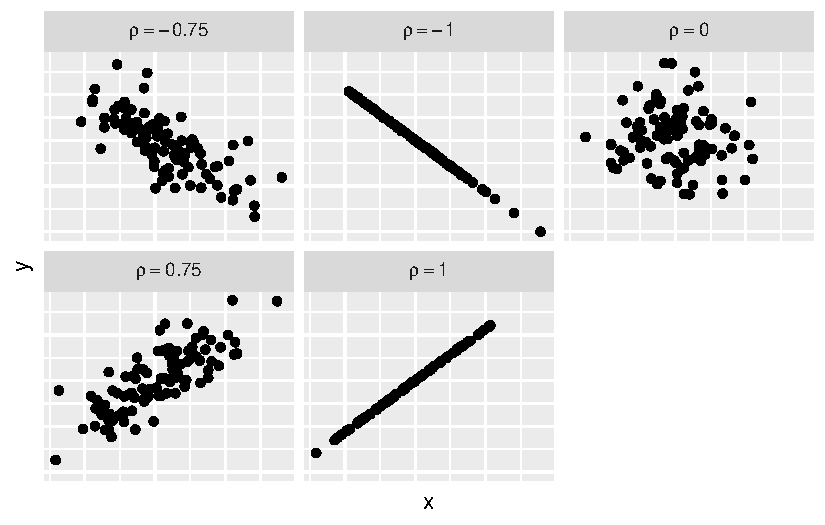
\includegraphics[width=0.8\textwidth,height=\textheight]{index_files/figure-pdf/correlation2-1.pdf}

}

\caption{Differing levels of correlation between variables.}

\end{figure}%

The correlation coefficient can be computed in R using the \texttt{cor}
function as follows:

\begin{Shaded}
\begin{Highlighting}[]
\FunctionTok{cor}\NormalTok{(evals.scores}\SpecialCharTok{$}\NormalTok{score,evals.scores}\SpecialCharTok{$}\NormalTok{bty\_avg)}
\end{Highlighting}
\end{Shaded}

\begin{verbatim}
[1] 0.1871424
\end{verbatim}

Here, we are given a correlation coefficient of 0.187 for the
relationship between teaching (\texttt{score}) and beauty
(\texttt{bty\_avg}) scores. This suggests a rather \emph{weakly
positive} linear relationship between the two variables. There is some
subjective interpretation surrounding correlation coefficients not very
close to -1, 0, 1. The table below provides a rough guide as to the
verbal interpretation of a correlation coefficient.

\begin{longtable}[]{@{}
  >{\raggedright\arraybackslash}p{(\columnwidth - 2\tabcolsep) * \real{0.4167}}
  >{\raggedright\arraybackslash}p{(\columnwidth - 2\tabcolsep) * \real{0.5833}}@{}}
\toprule\noalign{}
\begin{minipage}[b]{\linewidth}\raggedright
Correlation coefficient
\end{minipage} & \begin{minipage}[b]{\linewidth}\raggedright
Verbal interpretation
\end{minipage} \\
\midrule\noalign{}
\endhead
\bottomrule\noalign{}
\endlastfoot
0.90 to 1.00 (-0.90 to -1.00) & Very strong positive (negative)
correlation \\
0.70 to 0.90 (-0.70 to -0.90) & Strong positive (negative)
correlation \\
0.50 to 0.70 (-0.50 to -0.70) & Moderate positive (negative)
correlation \\
0.30 to 0.50 (-0.30 to -0.50) & Weak positive (negative) correlation \\
0.00 to 0.30 (0.00 to -0.30) & Very weak positive (negative)
correlation \\
\end{longtable}

The next step in our exploratory data analysis is to visualise the data
using appropriate plotting techniques. Here, a scatterplot is
appropriate since both \texttt{score} and \texttt{bty\_avg} are
numerical variables:

\begin{Shaded}
\begin{Highlighting}[]
\FunctionTok{ggplot}\NormalTok{(evals.scores, }\FunctionTok{aes}\NormalTok{(}\AttributeTok{x =}\NormalTok{ bty\_avg, }\AttributeTok{y =}\NormalTok{ score)) }\SpecialCharTok{+}
  \FunctionTok{geom\_point}\NormalTok{() }\SpecialCharTok{+}
  \FunctionTok{labs}\NormalTok{(}\AttributeTok{x =} \StringTok{"Beauty Score"}\NormalTok{, }\AttributeTok{y =} \StringTok{"Teaching Score"}\NormalTok{, }\AttributeTok{title =} \StringTok{"Relationship of teaching and beauty scores"}\NormalTok{)}
\end{Highlighting}
\end{Shaded}

\begin{figure}[H]

{\centering 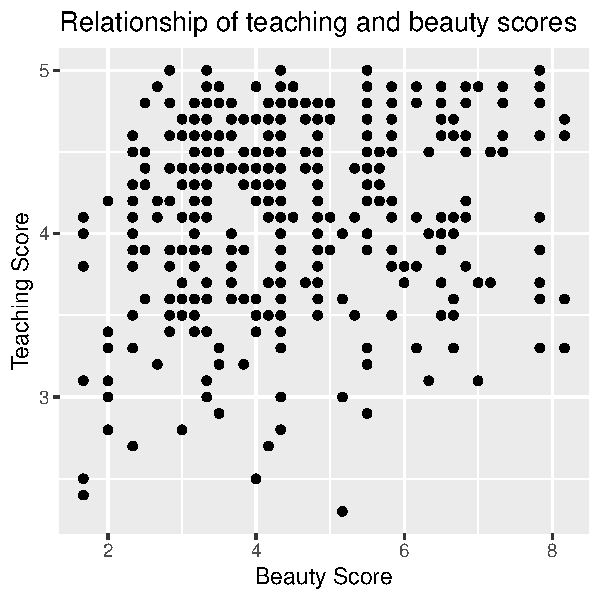
\includegraphics{index_files/figure-pdf/unnamed-chunk-4-1.pdf}

}

\caption{Relationship between teaching and beauty scores.}

\end{figure}%

\begin{tcolorbox}[enhanced jigsaw, leftrule=.75mm, opacityback=0, colbacktitle=quarto-callout-note-color!10!white, left=2mm, rightrule=.15mm, colframe=quarto-callout-note-color-frame, colback=white, coltitle=black, breakable, bottomtitle=1mm, title=\textcolor{quarto-callout-note-color}{\faInfo}\hspace{0.5em}{Note}, toprule=.15mm, titlerule=0mm, toptitle=1mm, bottomrule=.15mm, opacitybacktitle=0.6, arc=.35mm]

The outcome variable should always be plotted on the y-axis.

\end{tcolorbox}

What can we observe from the scatterplot? Well, here it can be hard to
see the weakly positive linear relationship suggested by the correlation
coefficient (0.187), which is why our correlation coefficient is
considered \emph{very weak} in the verbal interpretation.

Additionally, as our numerical variables are averages of integers (or
whole numbers), a lot of the values will be plotted on top of one
another. This is often referred to as \textbf{over-plotting}, and can be
alleviated by slightly nudging (\textbf{jittering}) the points in a
random direction (This can be done by adding a\texttt{geom\_jitter()}
layer in our ggplot object). For example, let's look at the three points
in the top-right of the scatterplot that have a beauty score slightly
less than 8. Are there really only three values plotted there, or are
there more that we cannot see due to over-plotting? Let's find out by
adding some jitter to the plot:

\begin{figure}[H]

{\centering 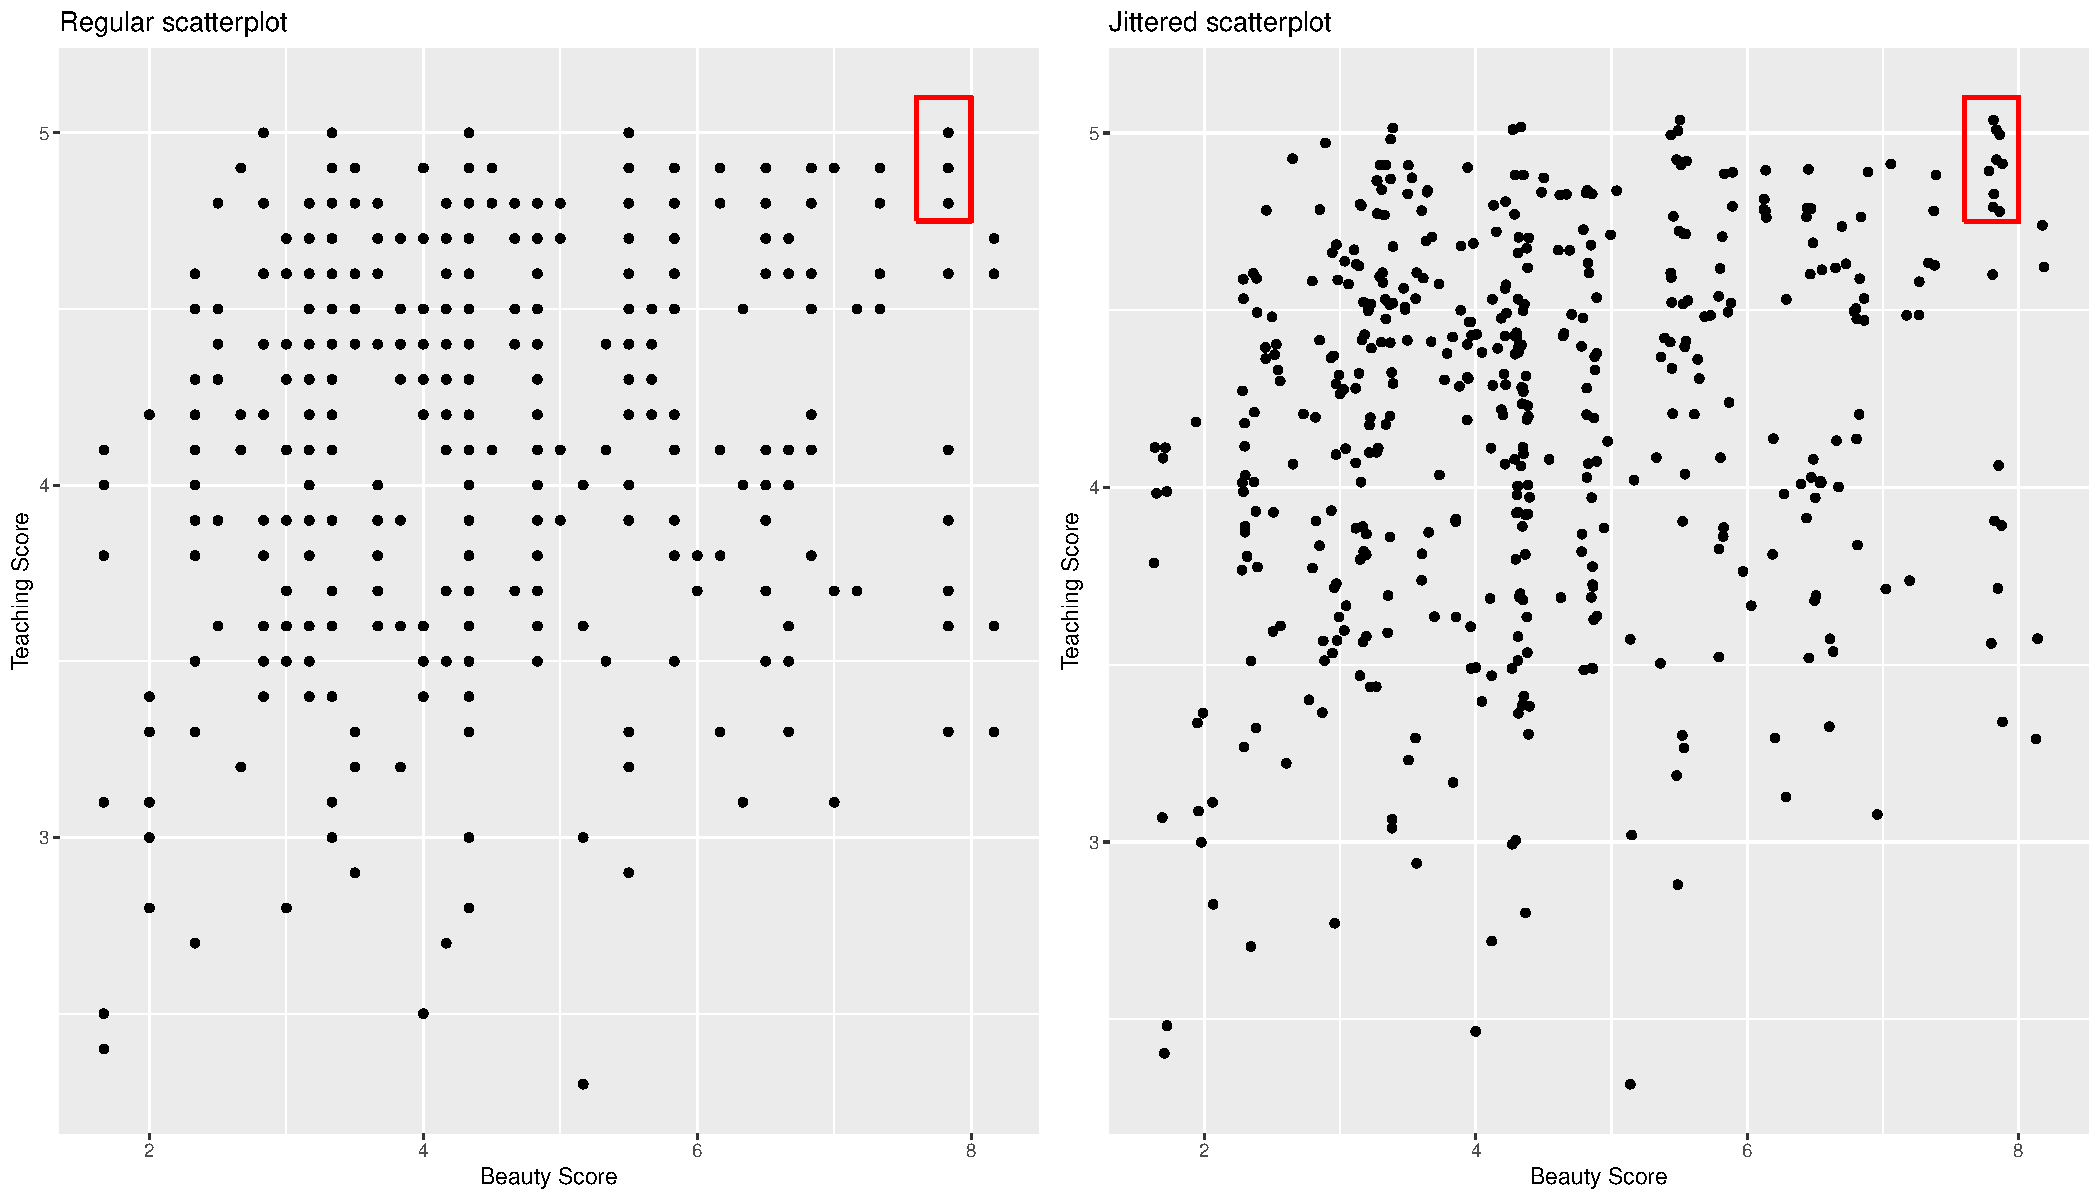
\includegraphics{index_files/figure-pdf/correlation5-1.pdf}

}

\caption{Comparing regular and jittered scatterplots.}

\end{figure}%

From the jittered scatterplot we can see that:

\begin{enumerate}
\def\labelenumi{\arabic{enumi}.}
\tightlist
\item
  There are actually more than just three points plotted in the
  top-right; and
\item
  There are more instructors with a beauty score between 3 and 4.5 than
  originally appears due to over-plotting.
\end{enumerate}

\begin{tcolorbox}[enhanced jigsaw, leftrule=.75mm, opacityback=0, colbacktitle=quarto-callout-note-color!10!white, left=2mm, rightrule=.15mm, colframe=quarto-callout-note-color-frame, colback=white, coltitle=black, breakable, bottomtitle=1mm, title=\textcolor{quarto-callout-note-color}{\faInfo}\hspace{0.5em}{Note}, toprule=.15mm, titlerule=0mm, toptitle=1mm, bottomrule=.15mm, opacitybacktitle=0.6, arc=.35mm]

Jittering does not actually change the values within a data set, it is
merely a tool for visualisation purposes. Hence, we shall continue on
with plotting the original data.

\end{tcolorbox}

\subsection{Formal analysis}\label{formal-analysis}

After completing an exploratory data analysis the next step is to
perform a \textbf{formal analysis} on the data. This involves
constructing an appropriate statistical model from the information
gathered during the exploratory data analysis step. Here, we shall be
fitting a simple linear regression model to the data on teaching and
beauty scores, where our objective is to acquire the best fitting
regression line. This is done by finding estimates of the intercept
(\(\alpha\)) and slope (\(\beta\)) which give us the best-fitting line
to the data. This can be done in R using the \texttt{lm} function:

\begin{Shaded}
\begin{Highlighting}[]
\NormalTok{model }\OtherTok{\textless{}{-}} \FunctionTok{lm}\NormalTok{(score }\SpecialCharTok{\textasciitilde{}}\NormalTok{ bty\_avg, }\AttributeTok{data =}\NormalTok{ evals.scores)}
\FunctionTok{tab\_model}\NormalTok{(model,}\AttributeTok{show.ci =}\NormalTok{ F)}
\end{Highlighting}
\end{Shaded}

\begin{longtable}[]{@{}ccc@{}}
\toprule\noalign{}
\endhead
\bottomrule\noalign{}
\endlastfoot
~ & \multicolumn{2}{c@{}}{%
score} \\
Predictors & Estimates & p \\
(Intercept) & 3.88 & \textbf{\textless0.001} \\
bty avg & 0.07 & \textbf{\textless0.001} \\
Observations & \multicolumn{2}{l@{}}{%
463} \\
R\textsuperscript{2} / R\textsuperscript{2} adjusted &
\multicolumn{2}{l@{}}{%
0.035 / 0.033} \\
\end{longtable}

We have summarised the fitted model using the \texttt{tab\_model}
function from the \texttt{sjPlot} library (we have omitted confidence
intervals for now). This tells us that our best-fitting line to the data
is:

\[\widehat{\text{score}} = \widehat{\alpha} + \widehat{\beta} x_i = 3.88 + 0.07 \cdot \mathrm{bty\_avg},\]
where

\begin{itemize}
\tightlist
\item
  \(\widehat{\alpha} = 3.88\) is the intercept coefficient and means
  that, for any instructor with a \texttt{bty\_avg\ =\ 0}, their average
  teaching \texttt{score} would be 3.88. Note that
  \texttt{bty\_avg\ =\ 0} is not actually possible as \texttt{bty\_avg}
  is an average of beauty scores ranging between 1 and 10.
\item
  \(\widehat{\beta} = 0.07\) is the slope coefficient associated with
  the exploratory variable \texttt{bty\_avg}, and summarises the
  relationship between \texttt{score} and \texttt{bty\_avg}. That is, as
  \texttt{bty\_avg} increases, so does \texttt{score}, such that

  \begin{itemize}
  \tightlist
  \item
    For every 1 unit increase in \texttt{bty\_avg}, there is an
    associated increase of, on average, 0.06664 units of \texttt{score}.
  \end{itemize}
\end{itemize}

\begin{tcolorbox}[enhanced jigsaw, leftrule=.75mm, opacityback=0, colbacktitle=quarto-callout-note-color!10!white, left=2mm, rightrule=.15mm, colframe=quarto-callout-note-color-frame, colback=white, coltitle=black, breakable, bottomtitle=1mm, title=\textcolor{quarto-callout-note-color}{\faInfo}\hspace{0.5em}{Note}, toprule=.15mm, titlerule=0mm, toptitle=1mm, bottomrule=.15mm, opacitybacktitle=0.6, arc=.35mm]

The \texttt{broom} library is another alternative to \texttt{sjPlot}
that allow us to visualize linear model output in a tidy way. For
example, we can ask for a model summary using the \texttt{tidy} function
that will return the output in a \texttt{data.frame} format:

\begin{Shaded}
\begin{Highlighting}[]
\FunctionTok{library}\NormalTok{(broom)}
\FunctionTok{tidy}\NormalTok{(model)}
\end{Highlighting}
\end{Shaded}

\begin{verbatim}
# A tibble: 2 x 5
  term        estimate std.error statistic   p.value
  <chr>          <dbl>     <dbl>     <dbl>     <dbl>
1 (Intercept)   3.88      0.0761     51.0  1.56e-191
2 bty_avg       0.0666    0.0163      4.09 5.08e-  5
\end{verbatim}

\end{tcolorbox}

Finally, we can superimpose our best-fitting line onto our scatterplot
to see how it fits through the points using the \texttt{geom\_smooth}
function as follows:

\begin{Shaded}
\begin{Highlighting}[]
\FunctionTok{ggplot}\NormalTok{(evals.scores, }\FunctionTok{aes}\NormalTok{(}\AttributeTok{x =}\NormalTok{ bty\_avg, }\AttributeTok{y =}\NormalTok{ score)) }\SpecialCharTok{+}
  \FunctionTok{geom\_point}\NormalTok{() }\SpecialCharTok{+}
  \FunctionTok{labs}\NormalTok{(}\AttributeTok{x =} \StringTok{"Beauty Score"}\NormalTok{, }\AttributeTok{y =} \StringTok{"Teaching Score"}\NormalTok{, }
       \AttributeTok{title =} \StringTok{"Relationship of teaching and beauty scores"}\NormalTok{) }\SpecialCharTok{+}
  \FunctionTok{geom\_smooth}\NormalTok{(}\AttributeTok{method =} \StringTok{"lm"}\NormalTok{, }\AttributeTok{se =} \ConstantTok{FALSE}\NormalTok{)}
\end{Highlighting}
\end{Shaded}

\begin{figure}[H]

{\centering 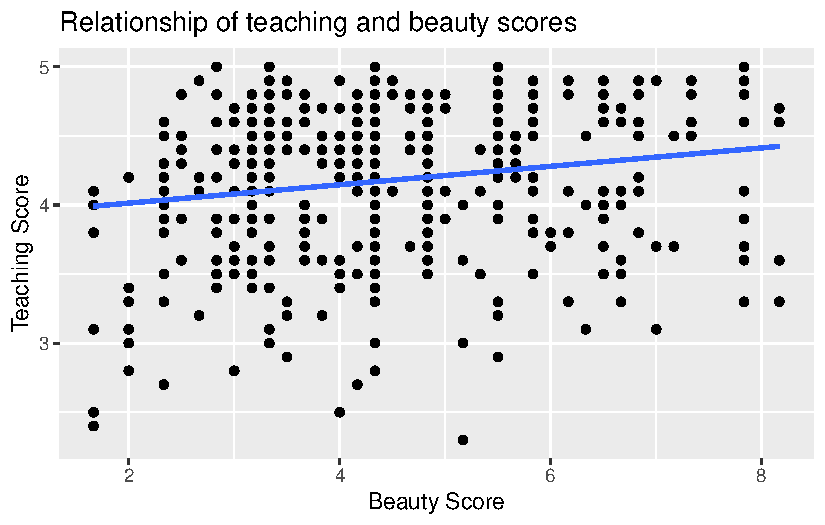
\includegraphics[width=0.5\textwidth,height=\textheight]{index_files/figure-pdf/lm2-1.pdf}

}

\caption{Relationship between teaching and beauty scores with regression
line superimposed.}

\end{figure}%

Now that we have fitted our simple linear regression model to the data,
how do we use it to obtain information on individual data points? This
can be done by looking at the \textbf{fitted values}. For example, let's
say we are interested in looking at the 21st instructor who has the
following teaching and beauty scores:

\begin{longtable}[]{@{}rr@{}}
\toprule\noalign{}
\texttt{score} & \texttt{bty\_avg} \\
\midrule\noalign{}
\endhead
\bottomrule\noalign{}
\endlastfoot
4.9 & 7.33 \\
\end{longtable}

What would the \texttt{score} be on our best-fitting line for this
instructor with a \texttt{bty\_avg} of 7.33? We simply plug the
instructor's \texttt{bty\_avg} into our regression model:

\[\widehat{\mbox{score}} = 3.88034 + 0.06664 \cdot \mbox{bty\_avg} = 3.88034 + 0.06664 \cdot 7.33 = 4.369,\]
The regression model gives our instructor a \texttt{score} of 4.369.
However, we know the \texttt{score} of the instructor is 4.9 meaning
that our model was out by 0.531. This is known as the \textbf{residual}
(\(\epsilon\)) and can be thought of as the error or \emph{lack of fit}
of the regression line. In this case, the residual is given by:

\[ \widehat{\epsilon} = y - \widehat{y} = 4.9 - 4.369 = 0.531.\]This is
essentially the distance between the fitted regression line and the
observed (true) value. This can be seen on the following scatterplot:

\begin{figure}[H]

{\centering 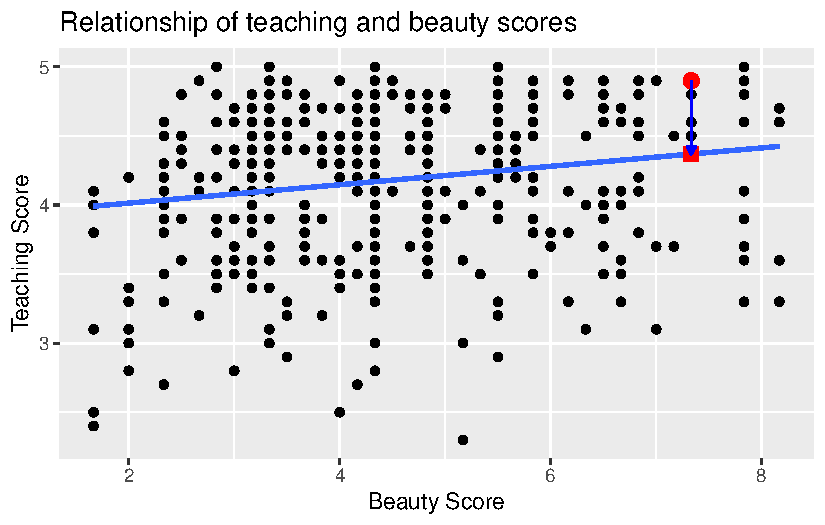
\includegraphics[width=0.5\textwidth,height=\textheight]{index_files/figure-pdf/lm3-1.pdf}

}

\caption{Example of observed value, fitted value, and residual.}

\end{figure}%

where

\begin{itemize}
\tightlist
\item
  the red circle is the observed (true) \texttt{score} (\(y=4.9\)) of
  the instructor;
\item
  the red square is the fitted value (\(\widehat{y} = 4.369\)) from the
  regression line; and
\item
  the blue arrow is the distance between the observed and fitted values,
  that is, the residual.
\end{itemize}

Residuals and fitted values can also be obtained directly from the
fitted model by typing \texttt{model\$fitted.values} and
\texttt{model\$residuals} respectively. We can appended these values to
our original data using the \texttt{mutate} function as follows:

\begin{Shaded}
\begin{Highlighting}[]
\NormalTok{ model\_output }\OtherTok{\textless{}{-}}\NormalTok{ evals.scores }\SpecialCharTok{\%\textgreater{}\%} 
   \FunctionTok{mutate}\NormalTok{(}\AttributeTok{score\_hat  =}\NormalTok{ model}\SpecialCharTok{$}\NormalTok{fitted.values,}
          \AttributeTok{residuals  =}\NormalTok{ model}\SpecialCharTok{$}\NormalTok{residuals)}
\NormalTok{ model\_output }\SpecialCharTok{\%\textgreater{}\%} \FunctionTok{slice}\NormalTok{(}\DecValTok{1}\SpecialCharTok{:}\DecValTok{6}\NormalTok{)}
\end{Highlighting}
\end{Shaded}

\begin{verbatim}
  score bty_avg score_hat  residuals
1   4.7       5  4.213523  0.4864769
2   4.1       5  4.213523 -0.1135231
3   3.9       5  4.213523 -0.3135231
4   4.8       5  4.213523  0.5864769
5   4.6       3  4.080249  0.5197509
6   4.3       3  4.080249  0.2197509
\end{verbatim}

\subsection{Assessing model fit}\label{assessing-model-fit}

When we fit a simple linear regression model there are five main
assumptions that we need to hold true in order for the model to be an
appropriate fit to the data. These assumptions are:

\begin{enumerate}
\def\labelenumi{\arabic{enumi}.}
\tightlist
\item
  The deterministic part of the model captures all the non-random
  structure in the data, i.e.~the residuals have mean zero.
\item
  The scale of the variability of the residuals is constant at all
  values of the explanatory variables (\emph{homoscedasticity}).
\item
  The residuals are normally distributed.
\item
  The residuals are independent.
\item
  The values of the explanatory variables are recorded without error.
\end{enumerate}

One way we can check our first assumption is to plot the residuals
(\texttt{residuals}) against the explanatory variable
(\texttt{bty\_avg}). From this we should be able to check that the
explanatory variable has a linear relationship with the outcome variable
(\texttt{score}). We can plot the residuals against our explanatory
variable using:

\begin{Shaded}
\begin{Highlighting}[]
\FunctionTok{ggplot}\NormalTok{(model\_output, }\FunctionTok{aes}\NormalTok{(}\AttributeTok{x =}\NormalTok{ bty\_avg, }\AttributeTok{y =}\NormalTok{ residuals)) }\SpecialCharTok{+}
  \FunctionTok{geom\_point}\NormalTok{() }\SpecialCharTok{+}
  \FunctionTok{labs}\NormalTok{(}\AttributeTok{x =} \StringTok{"Beauty Score"}\NormalTok{, }\AttributeTok{y =} \StringTok{"Residual"}\NormalTok{) }\SpecialCharTok{+}
  \FunctionTok{geom\_hline}\NormalTok{(}\AttributeTok{yintercept =} \DecValTok{0}\NormalTok{, }\AttributeTok{col =} \StringTok{"blue"}\NormalTok{, }\AttributeTok{linewidth =} \DecValTok{1}\NormalTok{)}
\end{Highlighting}
\end{Shaded}

\begin{figure}[H]

{\centering 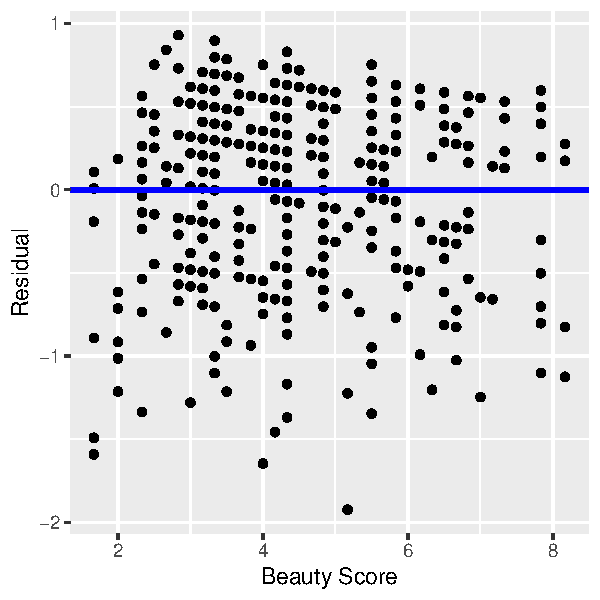
\includegraphics{index_files/figure-pdf/unnamed-chunk-7-1.pdf}

}

\caption{Residuals against beauty score.}

\end{figure}%

Ideally, for the first assumption to hold we should observe the
following:

\begin{itemize}
\tightlist
\item
  There should be no systematic pattern, i.e.~the residuals should
  appear randomly scattered.
\item
  The residuals should have mean zero. That is, they should be evenly
  scattered above and below the zero line. This is because the
  regression model will overestimate some of the fitted values, but it
  will also underestimate some, and hence, on average, they should even
  out to have mean zero.
\end{itemize}

Another way in which we can examine our first two assumptions is by
plotting the residuals against the fitted values.

The \texttt{performance} package allows us to do so via the
\texttt{check\_model()} function as follows:

\begin{Shaded}
\begin{Highlighting}[]
\FunctionTok{check\_model}\NormalTok{(model,}\AttributeTok{check =} \FunctionTok{c}\NormalTok{(}\StringTok{"homogeneity"}\NormalTok{,}\StringTok{"linearity"}\NormalTok{))}
\end{Highlighting}
\end{Shaded}

\begin{figure}[H]

{\centering 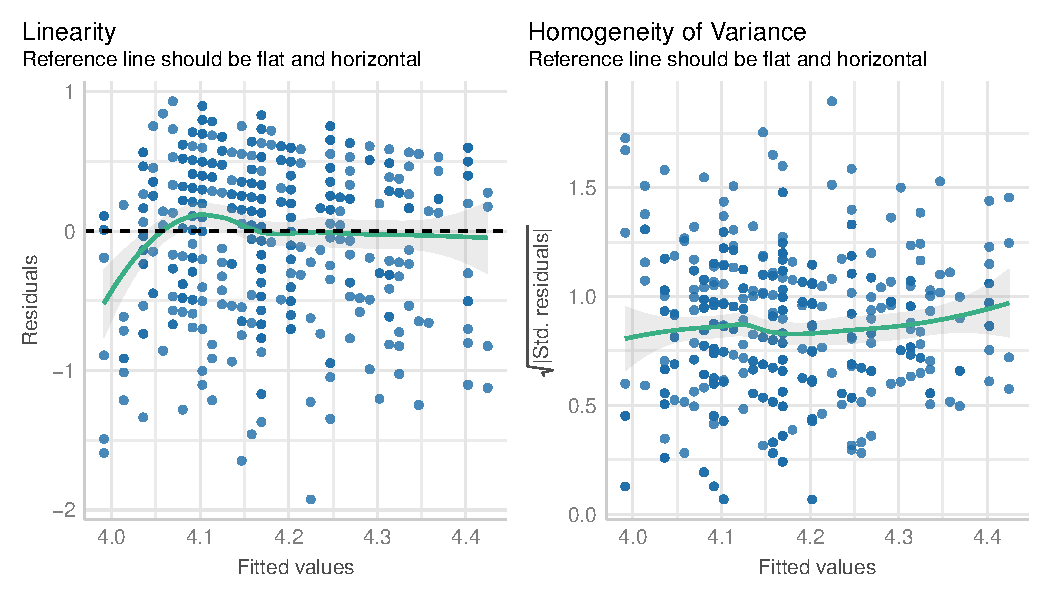
\includegraphics{index_files/figure-pdf/unnamed-chunk-8-1.pdf}

}

\caption{Residuals against fitted values.}

\end{figure}%

Here we have asked to \texttt{check\_model} function to check the
\emph{homoscedasticity}and linearity assumptions by setting
\texttt{check\ =\ \ c("homogeneity","linearity")} . From the plot of the
residuals against the fitted values we want to examine whether:

\begin{itemize}
\tightlist
\item
  The residuals have mean zero (left plot).
\item
  If the residuals have constant variance across all levels of the
  fitted values. That is, the range (or spread) of the residuals should
  be similar across all levels of the fitted values and display no
  obvious changes in variability (right plot).
\end{itemize}

These two assumptions seems to hold for our model. To assess our third
assumption that the residuals are normally distributed we can simply
plot a histogram of the residuals and compare the theoretical quantiles
of the normal distribution against the sample quantiles.

\begin{Shaded}
\begin{Highlighting}[]
\FunctionTok{check\_model}\NormalTok{(model,}\AttributeTok{check =} \FunctionTok{c}\NormalTok{(}\StringTok{"normality"}\NormalTok{,}\StringTok{"qq"}\NormalTok{))}
\end{Highlighting}
\end{Shaded}

\begin{figure}[H]

{\centering 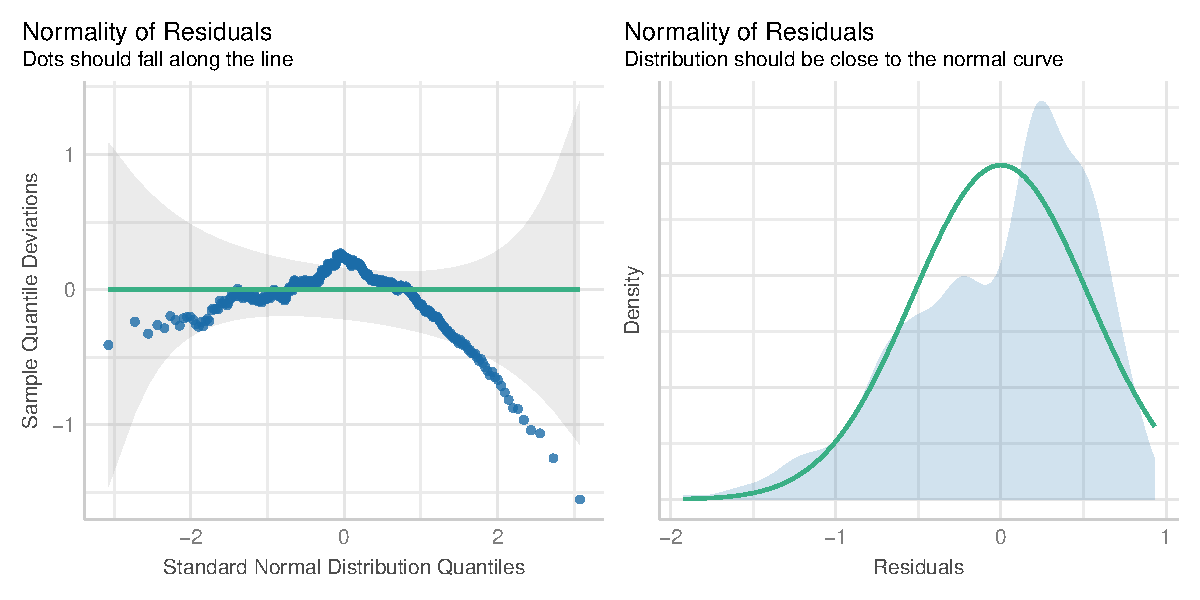
\includegraphics{index_files/figure-pdf/lm9-1.pdf}

}

\caption{QQ-plot and Histogram of residuals.}

\end{figure}%

Ideally, for the assumption of normally distributed residuals, the
histogram should be bell-shaped and centred at zero, i.e.~the residuals
have mean zero. However, in practice this will almost never be the case,
and as such, like the plots of the residuals, there is some subjectivity
in whether you believe the assumptions hold. For instance, here we can
see that the histogram is slightly skewed to the left in that the
distribution has a longer tail to the left. We can also assess these
assumption by comparing the theoretical quantiles of the normal
distribution against the sample quantiles. If the normality assumption
holds, then we expect that most of the dots should fall along the line.
However this seems not to be the case and while the histogram appears to
be relatively symmetrical and bell-shaped, the assumption of normally
distributed random errors seems dubious.

Note that we can get similar diagnostic plots using the
\texttt{plot\_model} function from the \texttt{sjPlot} package by adding
the \texttt{type=\textquotesingle{}diag\textquotesingle{}} option. This
will produce a list of plots that can be accessed as follows:

\begin{Shaded}
\begin{Highlighting}[]
\NormalTok{diag\_plots }\OtherTok{=} \FunctionTok{plot\_model}\NormalTok{(model,}\AttributeTok{type=}\StringTok{\textquotesingle{}diag\textquotesingle{}}\NormalTok{)}

\CommentTok{\# QQ plot}
\NormalTok{diag\_plots[[}\DecValTok{1}\NormalTok{]]}
\end{Highlighting}
\end{Shaded}

\begin{center}
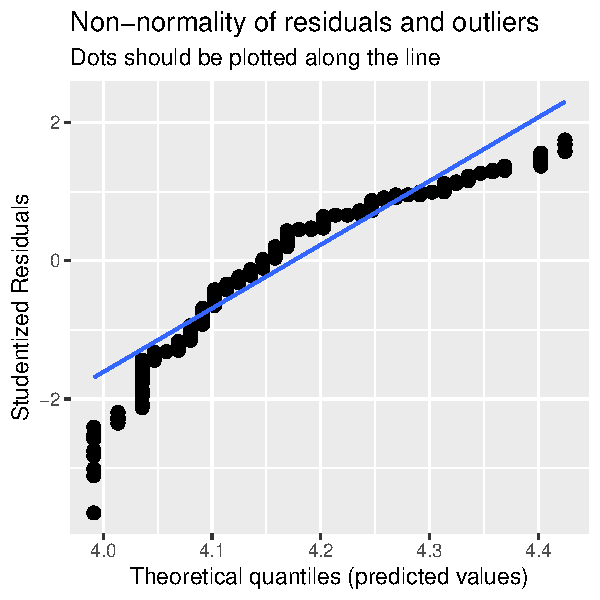
\includegraphics{index_files/figure-pdf/unnamed-chunk-9-1.pdf}
\end{center}

\begin{Shaded}
\begin{Highlighting}[]
\CommentTok{\# Histrogram/density plot}
\NormalTok{diag\_plots[[}\DecValTok{2}\NormalTok{]]}
\end{Highlighting}
\end{Shaded}

\begin{center}
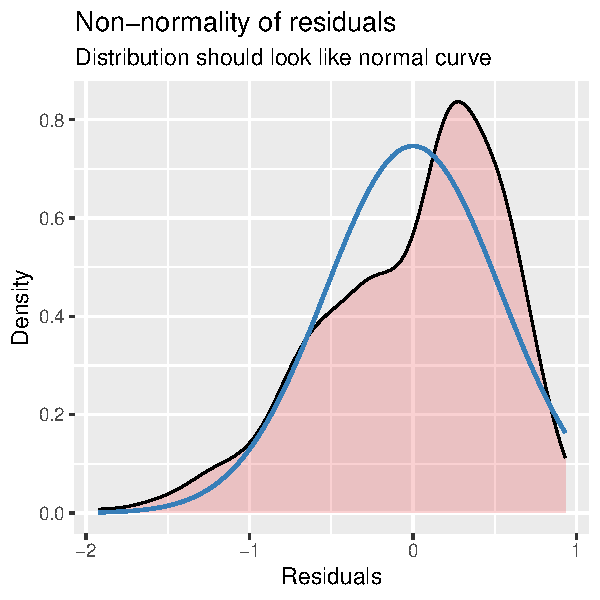
\includegraphics{index_files/figure-pdf/unnamed-chunk-9-2.pdf}
\end{center}

\begin{Shaded}
\begin{Highlighting}[]
\CommentTok{\# Residuals vs fitted values}
\NormalTok{diag\_plots[[}\DecValTok{3}\NormalTok{]]}
\end{Highlighting}
\end{Shaded}

\begin{center}
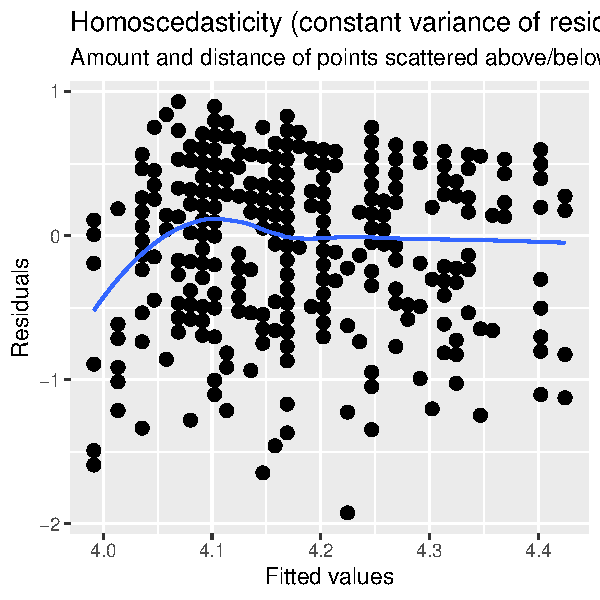
\includegraphics{index_files/figure-pdf/unnamed-chunk-9-3.pdf}
\end{center}

Finally, assumptions 4. and 5. are often justified on the basis of the
experimental context and are not formally examined.

\section{Simple linear regression with one categorical explanatory
variable}\label{simple-linear-regression-with-one-categorical-explanatory-variable}

Here, we will fit a simple linear regression model were the explanatory
variable is categorical. A \textbf{categorical variable} is a variable
of a fixed number of possible values, assigning units to particular
groups (or categories) based on qualitative properties.

We shall examine the \texttt{gapminder} data set (available from the
\texttt{gapminder} library) which you can download below:

This is a data set on life expectancy across various countries around
the world. We will explore life expectancy and its potential
differences:

\begin{itemize}
\tightlist
\item
  Between continents: Does life expectancy vary, on average, between the
  five continents of the world?; and
\item
  Within continents: Does life expectancy vary, on average, within the
  five continents of the world?
\end{itemize}

Thus, we will be looking at:

\begin{itemize}
\tightlist
\item
  life expectancy as our numerical outcome variable \(y\); and
\item
  the continent a country is within as our categorical variable \(x\).
\end{itemize}

\subsection{Exploratory data
analysis}\label{exploratory-data-analysis-1}

Let's examine a subset of the \texttt{gapminder} data set relating to
the year 2007. That is, we use the \texttt{filter} function to choose
only the observations pertaining to 2007, and then \texttt{select} the
variables we are interested in (remember to solve any conflicting
libraries using the \texttt{conflicts} package or refer to which package
each function is obtained from). Lastly we declare the \texttt{country}
and \texttt{continent} continent variables as factors using the
\texttt{mutate} function:

\begin{Shaded}
\begin{Highlighting}[]
\NormalTok{gapminder }\OtherTok{\textless{}{-}} \FunctionTok{read.csv}\NormalTok{(}\StringTok{"gapminder.csv"}\NormalTok{)}

\NormalTok{gapminder2007 }\OtherTok{\textless{}{-}}\NormalTok{ gapminder }\SpecialCharTok{\%\textgreater{}\%}
\NormalTok{  dplyr}\SpecialCharTok{::}\FunctionTok{filter}\NormalTok{(year }\SpecialCharTok{==} \DecValTok{2007}\NormalTok{) }\SpecialCharTok{\%\textgreater{}\%} 
\NormalTok{  dplyr}\SpecialCharTok{::}\FunctionTok{select}\NormalTok{(country, continent, lifeExp) }\SpecialCharTok{\%\textgreater{}\%}
  \FunctionTok{mutate}\NormalTok{(}\AttributeTok{country  =} \FunctionTok{as.factor}\NormalTok{(country),}
         \AttributeTok{continent =} \FunctionTok{as.factor}\NormalTok{(continent))}
\end{Highlighting}
\end{Shaded}

The new data set can be examined using either the \texttt{View} or
\texttt{glimpse} functions, i.e.

\begin{Shaded}
\begin{Highlighting}[]
\FunctionTok{glimpse}\NormalTok{(gapminder2007)}
\end{Highlighting}
\end{Shaded}

\begin{verbatim}
Rows: 142
Columns: 3
$ country   <fct> "Afghanistan", "Albania", "Algeria", "Angola", "Argentina", ~
$ continent <fct> Asia, Europe, Africa, Africa, Americas, Oceania, Europe, Asi~
$ lifeExp   <dbl> 43.828, 76.423, 72.301, 42.731, 75.320, 81.235, 79.829, 75.6~
\end{verbatim}

Here, we can see that both \texttt{country} and \texttt{continent} are
factors (\texttt{fct}), which is a way in how R stores categorical
variables. Similarly to our previous exploratory data analysis, we can
obtain summary statistics using the \texttt{skim} function. First, let's
take a look at the life expectancy (\texttt{lifeExp}) and
\texttt{continent} variables:

\begin{Shaded}
\begin{Highlighting}[]
\NormalTok{gapminder2007 }\SpecialCharTok{\%\textgreater{}\%} 
  \FunctionTok{select}\NormalTok{(continent, lifeExp) }\SpecialCharTok{\%\textgreater{}\%} 
  \FunctionTok{skim}\NormalTok{()}
\end{Highlighting}
\end{Shaded}

\begin{longtable}[]{@{}ll@{}}
\caption{Data summary}\tabularnewline
\toprule\noalign{}
\endfirsthead
\endhead
\bottomrule\noalign{}
\endlastfoot
Name & Piped data \\
Number of rows & 142 \\
Number of columns & 2 \\
\_\_\_\_\_\_\_\_\_\_\_\_\_\_\_\_\_\_\_\_\_\_\_ & \\
Column type frequency: & \\
factor & 1 \\
numeric & 1 \\
\_\_\_\_\_\_\_\_\_\_\_\_\_\_\_\_\_\_\_\_\_\_\_\_ & \\
Group variables & None \\
\end{longtable}

\textbf{Variable type: factor}

\begin{longtable}[]{@{}
  >{\raggedright\arraybackslash}p{(\columnwidth - 10\tabcolsep) * \real{0.1556}}
  >{\raggedleft\arraybackslash}p{(\columnwidth - 10\tabcolsep) * \real{0.1111}}
  >{\raggedleft\arraybackslash}p{(\columnwidth - 10\tabcolsep) * \real{0.1556}}
  >{\raggedright\arraybackslash}p{(\columnwidth - 10\tabcolsep) * \real{0.0889}}
  >{\raggedleft\arraybackslash}p{(\columnwidth - 10\tabcolsep) * \real{0.1000}}
  >{\raggedright\arraybackslash}p{(\columnwidth - 10\tabcolsep) * \real{0.3889}}@{}}
\toprule\noalign{}
\begin{minipage}[b]{\linewidth}\raggedright
skim\_variable
\end{minipage} & \begin{minipage}[b]{\linewidth}\raggedleft
n\_missing
\end{minipage} & \begin{minipage}[b]{\linewidth}\raggedleft
complete\_rate
\end{minipage} & \begin{minipage}[b]{\linewidth}\raggedright
ordered
\end{minipage} & \begin{minipage}[b]{\linewidth}\raggedleft
n\_unique
\end{minipage} & \begin{minipage}[b]{\linewidth}\raggedright
top\_counts
\end{minipage} \\
\midrule\noalign{}
\endhead
\bottomrule\noalign{}
\endlastfoot
continent & 0 & 1 & FALSE & 5 & Afr: 52, Asi: 33, Eur: 30, Ame: 25 \\
\end{longtable}

\textbf{Variable type: numeric}

\begin{longtable}[]{@{}
  >{\raggedright\arraybackslash}p{(\columnwidth - 20\tabcolsep) * \real{0.1647}}
  >{\raggedleft\arraybackslash}p{(\columnwidth - 20\tabcolsep) * \real{0.1176}}
  >{\raggedleft\arraybackslash}p{(\columnwidth - 20\tabcolsep) * \real{0.1647}}
  >{\raggedleft\arraybackslash}p{(\columnwidth - 20\tabcolsep) * \real{0.0706}}
  >{\raggedleft\arraybackslash}p{(\columnwidth - 20\tabcolsep) * \real{0.0706}}
  >{\raggedleft\arraybackslash}p{(\columnwidth - 20\tabcolsep) * \real{0.0706}}
  >{\raggedleft\arraybackslash}p{(\columnwidth - 20\tabcolsep) * \real{0.0706}}
  >{\raggedleft\arraybackslash}p{(\columnwidth - 20\tabcolsep) * \real{0.0706}}
  >{\raggedleft\arraybackslash}p{(\columnwidth - 20\tabcolsep) * \real{0.0706}}
  >{\raggedleft\arraybackslash}p{(\columnwidth - 20\tabcolsep) * \real{0.0588}}
  >{\raggedright\arraybackslash}p{(\columnwidth - 20\tabcolsep) * \real{0.0706}}@{}}
\toprule\noalign{}
\begin{minipage}[b]{\linewidth}\raggedright
skim\_variable
\end{minipage} & \begin{minipage}[b]{\linewidth}\raggedleft
n\_missing
\end{minipage} & \begin{minipage}[b]{\linewidth}\raggedleft
complete\_rate
\end{minipage} & \begin{minipage}[b]{\linewidth}\raggedleft
mean
\end{minipage} & \begin{minipage}[b]{\linewidth}\raggedleft
sd
\end{minipage} & \begin{minipage}[b]{\linewidth}\raggedleft
p0
\end{minipage} & \begin{minipage}[b]{\linewidth}\raggedleft
p25
\end{minipage} & \begin{minipage}[b]{\linewidth}\raggedleft
p50
\end{minipage} & \begin{minipage}[b]{\linewidth}\raggedleft
p75
\end{minipage} & \begin{minipage}[b]{\linewidth}\raggedleft
p100
\end{minipage} & \begin{minipage}[b]{\linewidth}\raggedright
hist
\end{minipage} \\
\midrule\noalign{}
\endhead
\bottomrule\noalign{}
\endlastfoot
lifeExp & 0 & 1 & 67.01 & 12.07 & 39.61 & 57.16 & 71.94 & 76.41 & 82.6 &
▂▃▃▆▇ \\
\end{longtable}

The summary output for the numerical outcome variable \texttt{lifeExp}
is the same as we have seen previously. However, for the categorical
variable \texttt{continent} we obtain:

\begin{itemize}
\tightlist
\item
  \texttt{n\_unique}: the number of levels (or categories) of the
  variable, i.e.~the number of continents.
\item
  \texttt{top\_counts}: the top counts from the top categories.
\item
  \texttt{ordered}: whether the variable is \emph{ordinal} or not. That
  is, whether or not the ordering of the categories matter.
\end{itemize}

\begin{tcolorbox}[enhanced jigsaw, leftrule=.75mm, opacityback=0, colbacktitle=quarto-callout-important-color!10!white, left=2mm, rightrule=.15mm, colframe=quarto-callout-important-color-frame, colback=white, coltitle=black, breakable, bottomtitle=1mm, title=\textcolor{quarto-callout-important-color}{\faExclamation}\hspace{0.5em}{Important}, toprule=.15mm, titlerule=0mm, toptitle=1mm, bottomrule=.15mm, opacitybacktitle=0.6, arc=.35mm]

It is important to always check your data after performing any kind of
manipulation. This helps ensure that you have not accidentally
overwritten a variable or introduced errors

\end{tcolorbox}

We can summarise any differences in life expectancy by continent by
taking a look at the median and mean life expectancies of each continent
using the \texttt{summarize} functions as follows:

\begin{Shaded}
\begin{Highlighting}[]
\NormalTok{lifeExp.continent }\OtherTok{\textless{}{-}}\NormalTok{ gapminder2007 }\SpecialCharTok{\%\textgreater{}\%}
  \FunctionTok{summarize}\NormalTok{(}\AttributeTok{median =} \FunctionTok{median}\NormalTok{(lifeExp), }\AttributeTok{mean =} \FunctionTok{mean}\NormalTok{(lifeExp),}\AttributeTok{.by =}\NormalTok{ continent)}
\NormalTok{lifeExp.continent}
\end{Highlighting}
\end{Shaded}

\begin{verbatim}
  continent  median     mean
1      Asia 72.3960 70.72848
2    Europe 78.6085 77.64860
3    Africa 52.9265 54.80604
4  Americas 72.8990 73.60812
5   Oceania 80.7195 80.71950
\end{verbatim}

Boxplots are often used when examining the distribution of a numerical
outcome variable across different levels of a categorical variable:

\begin{Shaded}
\begin{Highlighting}[]
\FunctionTok{ggplot}\NormalTok{(gapminder2007, }\FunctionTok{aes}\NormalTok{(}\AttributeTok{x =}\NormalTok{ continent, }\AttributeTok{y =}\NormalTok{ lifeExp)) }\SpecialCharTok{+}
  \FunctionTok{geom\_boxplot}\NormalTok{() }\SpecialCharTok{+}
  \FunctionTok{labs}\NormalTok{(}\AttributeTok{x =} \StringTok{"Continent"}\NormalTok{, }\AttributeTok{y =} \StringTok{"Life expectancy (years)"}\NormalTok{, }
       \AttributeTok{title =} \StringTok{"Life expectancy by continent"}\NormalTok{)}
\end{Highlighting}
\end{Shaded}

\begin{figure}[H]

{\centering 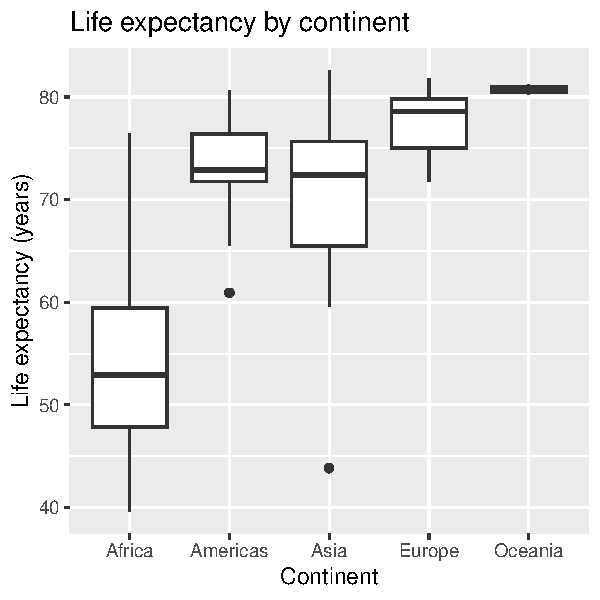
\includegraphics{index_files/figure-pdf/unnamed-chunk-13-1.pdf}

}

\caption{Life expectancy by continent in 2007.}

\end{figure}%

Here, we can see that the middle 50\% of the life expectancy
distribution of Africa is much smaller than, and does not overlap with,
the middle 50\% of the remaining four continents, while the country with
the highest life expectancy in Africa is less than all countries in
Oceania. Speaking of Oceania, there is almost no variability (or spread)
in life expectancy in this continent, however that may well be because
it consists of only two countries (Australia and New Zealand). There is
more variability in life expectancy in the continents of Africa and
Asia.

\subsection{Formal analysis}\label{formal-analysis-1}

When examining the relationship between a numerical outcome variable
\(y\) and a categorical explanatory variable \(x\), we are not just
looking to find the best-fitting line to the data as before, but are
examining relative differences to a baseline category. For example, the
table below displays the mean life expectancy of each continent, as well
as the differences between the means of each continent and Africa. Now,
in comparison with Africa we can see that the mean life expectancy of
the other continents is around 18-26 years greater than that of Africa.

\begin{longtable}[]{@{}lrr@{}}
\toprule\noalign{}
continent & mean & mean vs Africa \\
\midrule\noalign{}
\endhead
\bottomrule\noalign{}
\endlastfoot
Africa & 54.81 & 0.00 \\
Americas & 73.61 & 18.80 \\
Asia & 70.73 & 15.92 \\
Europe & 77.65 & 22.84 \\
Oceania & 80.72 & 25.91 \\
\end{longtable}

Now let us fit our regression model to the data, where \texttt{lifeExp}
is our outcome variable \(y\) and \texttt{continent} is our categorical
explanatory variable \(x\):

\begin{Shaded}
\begin{Highlighting}[]
\NormalTok{lifeExp.model }\OtherTok{\textless{}{-}} \FunctionTok{lm}\NormalTok{(lifeExp }\SpecialCharTok{\textasciitilde{}}\NormalTok{ continent, }\AttributeTok{data =}\NormalTok{ gapminder2007)}
\FunctionTok{tab\_model}\NormalTok{(lifeExp.model,}\AttributeTok{show.ci =}\NormalTok{ F)}
\end{Highlighting}
\end{Shaded}

\begin{longtable}[]{@{}ccc@{}}
\toprule\noalign{}
\endhead
\bottomrule\noalign{}
\endlastfoot
~ & \multicolumn{2}{c@{}}{%
life Exp} \\
Predictors & Estimates & p \\
(Intercept) & 54.81 & \textbf{\textless0.001} \\
continent {[}Americas{]} & 18.80 & \textbf{\textless0.001} \\
continent {[}Asia{]} & 15.92 & \textbf{\textless0.001} \\
continent {[}Europe{]} & 22.84 & \textbf{\textless0.001} \\
continent {[}Oceania{]} & 25.91 & \textbf{\textless0.001} \\
Observations & \multicolumn{2}{l@{}}{%
142} \\
R\textsuperscript{2} / R\textsuperscript{2} adjusted &
\multicolumn{2}{l@{}}{%
0.635 / 0.625} \\
\end{longtable}

We obtain five estimates: the \texttt{intercept} term and four others
relating to the continents (\texttt{continent\ {[}Americas{]}},
\texttt{continent\ {[}Asia{]}}, \texttt{continent\ {[}Europe{]}} and
\texttt{continent\ {[}Oceania{]}}), such that our regression equation is
given as:

\[\widehat{\text{life exp}} = \widehat{\alpha} + \widehat{\beta}_{\text{Amer}} \cdot \mathbb{I}_{\text{Amer}}(x) + \widehat{\beta}_{\text{Asia}} \cdot \mathbb{I}_{\text{Asia}}(x) + \widehat{\beta}_{\text{Euro}} \cdot \mathbb{I}_{\text{Euro}}(x) + \widehat{\beta}_{\text{Ocean}} \cdot \mathbb{I}_{\text{Ocean}}(x),\]
where

\begin{itemize}
\item
  the intercept \(\widehat{\alpha}\) is the mean life expectancy for our
  baseline category Africa;
\item
  \(\widehat{\beta}_{\text{continent}}\) is the difference in the mean
  life expectancy of a given continent relative to the baseline category
  Africa; and
\item
  \(\mathbb{I}_{\text{continent}}(x)\) is an indicator function such
  that

  \[\mathbb{I}_{\text{continent}}(x)=\left\{
              \begin{array}{ll}
                1 ~~~ \text{if country} ~ x ~ \text{is in the continent},\\
                0 ~~~ \text{Otherwise}.\\
              \end{array}
            \right.\]
\end{itemize}

Essentially, the estimates for each continent are known as
\emph{offsets} relative to the baseline category (Africa in this case).
For example, the mean life expectancy for Africa is simply equal to the
intercept term \(\widehat{\alpha} = 54.8\). However, the mean life
expectancy for Asia is:

\[\widehat{\alpha} + \widehat{\beta}_{\text{Asia}} \cdot \mathbb{I}_{\text{Asia}}(x) = 54.8 + 15.9 \cdot 1 = 70.7 \]

If we just look at a \(\widehat{\beta}_{\text{continent}}\) on their
own, then we would interpret these coefficients in relative terms with
respect to the baseline category. E.g., looking at
\(\widehat{\beta}_{\text{Asia}}=15.9\) , we would say that the life
expectancy in Asia is on average 15.9 years greater than in Africa.

\subsection{Assessing model fit}\label{assessing-model-fit-1}

What do the fitted values \(\widehat{y}\) and the residuals
\(y - \widehat{y}\) correspond to when we are dealing with a categorical
explanatory variable? Let's explore the \texttt{gapminder2007} data set
in order to understand how they work.

\begin{Shaded}
\begin{Highlighting}[]
\NormalTok{gapminder2007 }\SpecialCharTok{\%\textgreater{}\%} \FunctionTok{slice}\NormalTok{(}\DecValTok{1}\SpecialCharTok{:}\DecValTok{8}\NormalTok{)}
\end{Highlighting}
\end{Shaded}

\begin{verbatim}
      country continent lifeExp
1 Afghanistan      Asia  43.828
2     Albania    Europe  76.423
3     Algeria    Africa  72.301
4      Angola    Africa  42.731
5   Argentina  Americas  75.320
6   Australia   Oceania  81.235
7     Austria    Europe  79.829
8     Bahrain      Asia  75.635
\end{verbatim}

Here, we see the life expectancy of each country and the continent they
are from. For example, let's remember the life expectancies of
Afghanistan (43.8) and Bahrain (75.6). Now, we can obtain the fitted
values and residuals in the same way we did previously:

\begin{Shaded}
\begin{Highlighting}[]
\NormalTok{lifeExp.model\_output }\OtherTok{\textless{}{-}}\NormalTok{ gapminder2007 }\SpecialCharTok{\%\textgreater{}\%} 
  \FunctionTok{mutate}\NormalTok{(}\AttributeTok{lifeExp\_hat  =}\NormalTok{ lifeExp.model}\SpecialCharTok{$}\NormalTok{fitted.values,}
         \AttributeTok{residual =}\NormalTok{ lifeExp.model}\SpecialCharTok{$}\NormalTok{residuals)}

\NormalTok{lifeExp.model\_output }\SpecialCharTok{\%\textgreater{}\%} \FunctionTok{slice}\NormalTok{(}\DecValTok{1}\SpecialCharTok{:}\DecValTok{10}\NormalTok{)}
\end{Highlighting}
\end{Shaded}

\begin{table}

\caption{\label{tbl-lm_2output}Observed life expectancy values, fitted
values and residuals of a linear model fitted to the
\texttt{gapminder2007} data.}

\centering{

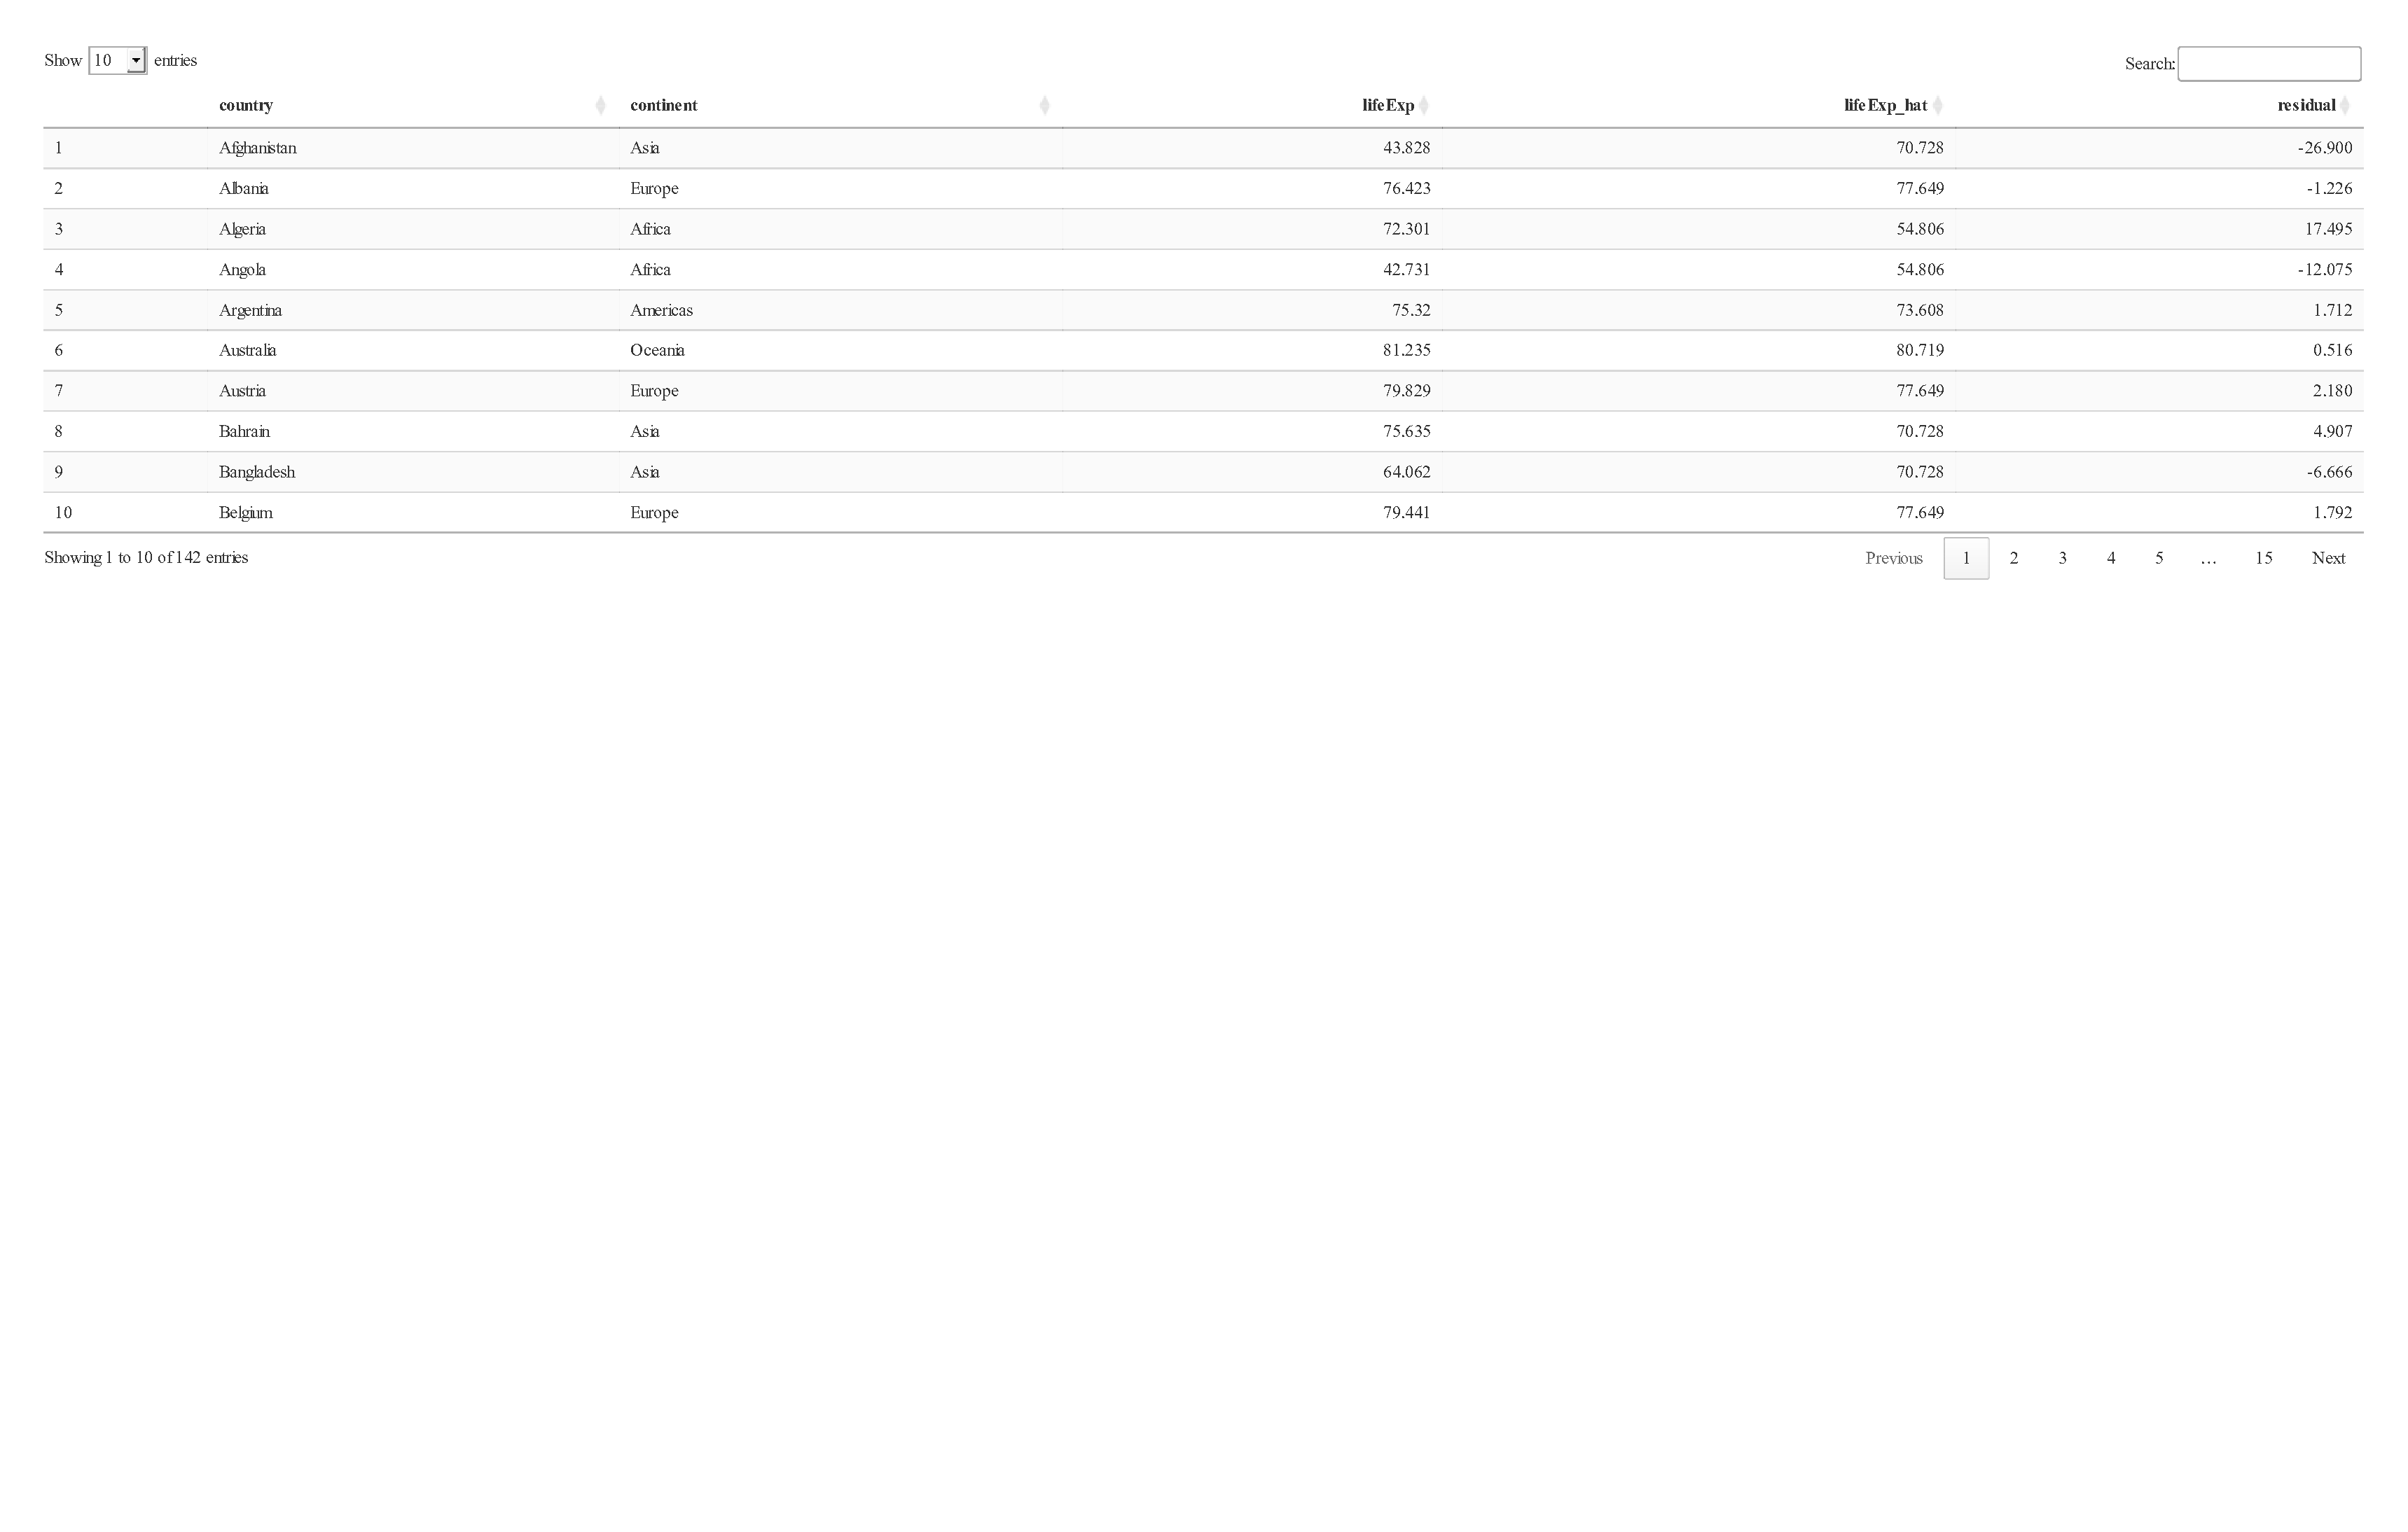
\includegraphics{index_files/figure-pdf/tbl-lm_2output-1.pdf}

}

\end{table}%

The first row of the regression table corresponds to the observed life
expectancy (\texttt{lifeExp}), fitted value (\texttt{lifeExp\_hat}) and
the residual error (\texttt{residual}) for Afghanistan. Here, we see
that the fitted value (\texttt{lifeExp\_hat\ =\ 70.7}) is much greater
than the life expectancy of Afghanistan (\texttt{lifeExp\ =\ 43.8}) with
a \texttt{residual\ =\ -26.9}. Now, for Bahrain (\texttt{ID\ =\ 8}) we
also have the same fitted value (\texttt{lifeExp\_hat\ =\ 70.7}) . This
is because the fitted values for each \texttt{country} correspond to the
mean life expectancy for that \texttt{continent} (you can use the search
box in Table~\ref{tbl-lm_2output} above and type \texttt{Asia} to show
only the observation in the Asia continent). Hence, all countries in
Africa have the fitted value \texttt{lifeExp\_hat\ =\ 70.7}, while all
countries in Europe have the fitted value
\texttt{lifeExp\_hat\ =\ 77.6}. The \texttt{residual} error in this case
is then how much a country deviates from the mean life expectancy of its
respective continent.

For assessing the assumptions surrounding the residuals for a
categorical explanatory variable, we can plot the residuals for each
continent:

\begin{Shaded}
\begin{Highlighting}[]
\FunctionTok{ggplot}\NormalTok{(lifeExp.model\_output, }\FunctionTok{aes}\NormalTok{(}\AttributeTok{x =}\NormalTok{ continent, }\AttributeTok{y =}\NormalTok{ residual)) }\SpecialCharTok{+}
  \FunctionTok{geom\_jitter}\NormalTok{(}\AttributeTok{width =} \FloatTok{0.1}\NormalTok{) }\SpecialCharTok{+} 
  \FunctionTok{labs}\NormalTok{(}\AttributeTok{x =} \StringTok{"Continent"}\NormalTok{, }\AttributeTok{y =} \StringTok{"Residual"}\NormalTok{) }\SpecialCharTok{+}
  \FunctionTok{geom\_hline}\NormalTok{(}\AttributeTok{yintercept =} \DecValTok{0}\NormalTok{, }\AttributeTok{col =} \StringTok{"blue"}\NormalTok{)}
\end{Highlighting}
\end{Shaded}

\begin{figure}[H]

{\centering 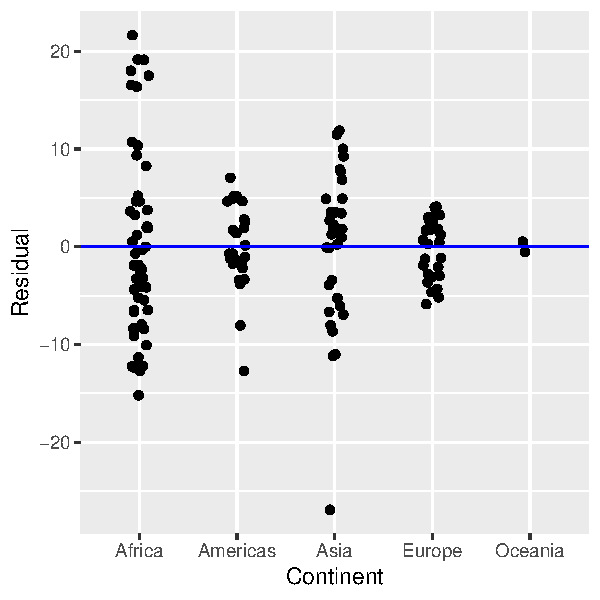
\includegraphics{index_files/figure-pdf/unnamed-chunk-19-1.pdf}

}

\caption{Residuals over continent.}

\end{figure}%

\begin{tcolorbox}[enhanced jigsaw, leftrule=.75mm, opacityback=0, colbacktitle=quarto-callout-note-color!10!white, left=2mm, rightrule=.15mm, colframe=quarto-callout-note-color-frame, colback=white, coltitle=black, breakable, bottomtitle=1mm, title=\textcolor{quarto-callout-note-color}{\faInfo}\hspace{0.5em}{Note}, toprule=.15mm, titlerule=0mm, toptitle=1mm, bottomrule=.15mm, opacitybacktitle=0.6, arc=.35mm]

We have jittered the points for each continent in order to see the
residuals for each country more clearly.

\end{tcolorbox}

Here, we see that there is an even spread of the residuals above and
below the zero line for each continent, and hence our assumption that
the residuals have mean zero appears valid. There is an outlier observed
for Asia with a large negative residual (relating to Afghanistan). We
could also check this by plotting the residuals agianst the fitted
values as follows:

\begin{Shaded}
\begin{Highlighting}[]
\FunctionTok{check\_model}\NormalTok{(lifeExp.model,}\AttributeTok{check=}\FunctionTok{c}\NormalTok{(}\StringTok{"homogeneity"}\NormalTok{,}\StringTok{"linearity"}\NormalTok{))}
\end{Highlighting}
\end{Shaded}

\begin{figure}[H]

{\centering 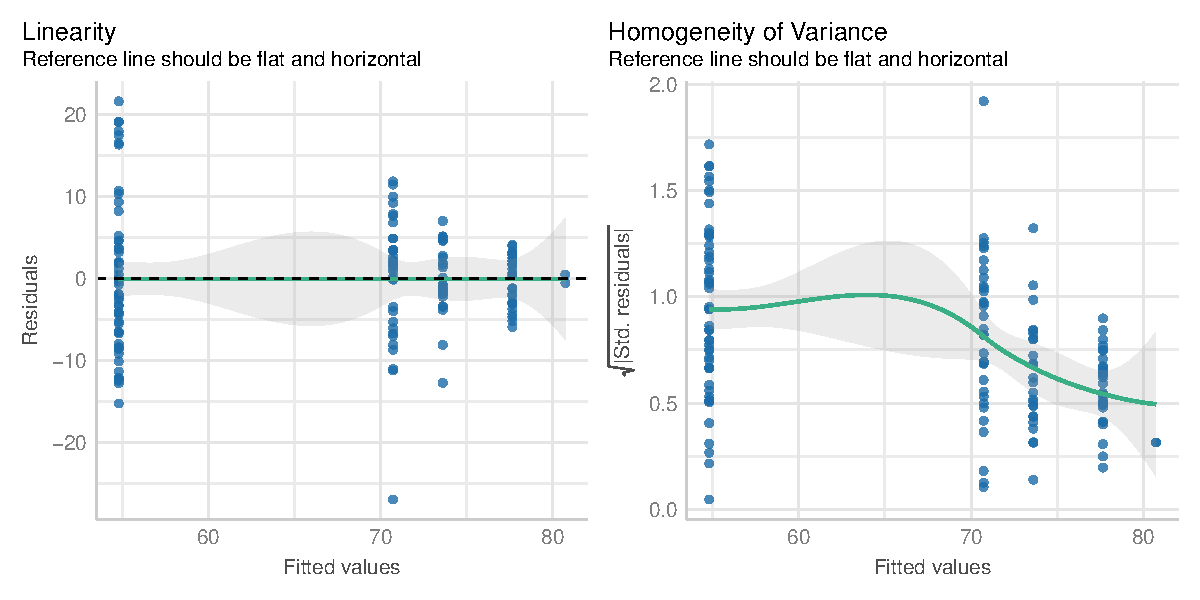
\includegraphics{index_files/figure-pdf/unnamed-chunk-20-1.pdf}

}

\caption{Residuals vs fitted values.}

\end{figure}%

Again, our assumption that the residuals have mean zero seems to hold.

\begin{tcolorbox}[enhanced jigsaw, leftrule=.75mm, opacityback=0, colbacktitle=quarto-callout-tip-color!10!white, left=2mm, rightrule=.15mm, colframe=quarto-callout-tip-color-frame, colback=white, coltitle=black, breakable, bottomtitle=1mm, title={Question}, toprule=.15mm, titlerule=0mm, toptitle=1mm, bottomrule=.15mm, opacitybacktitle=0.6, arc=.35mm]

What about the homoscedasticity assumption, is it valid?

\begin{itemize}
\tightlist
\item
  \begin{enumerate}
  \def\labelenumi{(\Alph{enumi})}
  \tightlist
  \item
    yes, residuals are not heteroscedastic\\
  \end{enumerate}
\item
  \begin{enumerate}
  \def\labelenumi{(\Alph{enumi})}
  \setcounter{enumi}{1}
  \tightlist
  \item
    no, there is an unbalanced number of residuals per country\\
  \end{enumerate}
\item
  \begin{enumerate}
  \def\labelenumi{(\Alph{enumi})}
  \setcounter{enumi}{2}
  \tightlist
  \item
    yes, residuals show an even spread across countries\\
  \end{enumerate}
\item
  \begin{enumerate}
  \def\labelenumi{(\Alph{enumi})}
  \setcounter{enumi}{3}
  \tightlist
  \item
    no, the spread of the residuals is not even across countries
  \end{enumerate}
\end{itemize}

\end{tcolorbox}

To check that the residual errors are normally distributed, we plot a
histogram and a QQplot of them:

\begin{Shaded}
\begin{Highlighting}[]
\FunctionTok{check\_model}\NormalTok{(lifeExp.model,}\AttributeTok{check=}\FunctionTok{c}\NormalTok{(}\StringTok{"qq"}\NormalTok{,}\StringTok{"normality"}\NormalTok{))}
\end{Highlighting}
\end{Shaded}

\begin{figure}[H]

{\centering 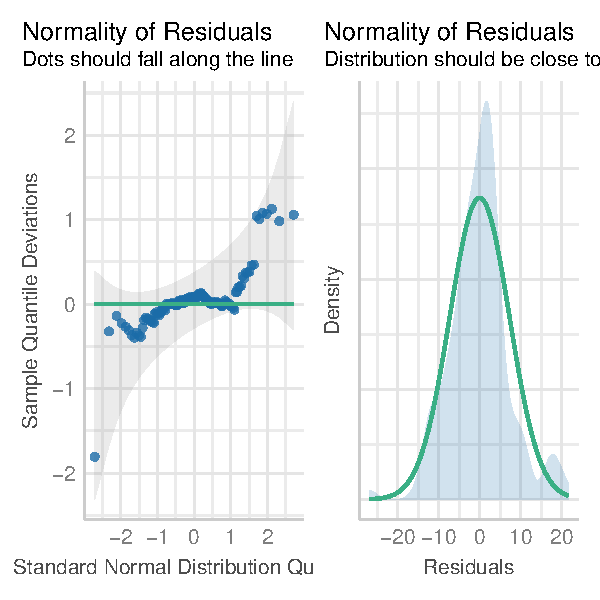
\includegraphics{index_files/figure-pdf/unnamed-chunk-22-1.pdf}

}

\caption{QQ-plot and Histogram of residuals.}

\end{figure}%

While some of the dots deviate from the flat line in the QQ plot, these
deviation occur at the tail where we have less data. Furthermore, the
histogram of the residuals are close to a bell-shaped and thus, the
assumption of normality seems valid.

\section{Multiple regression with two numerical explanatory
variables}\label{multiple-regression-with-two-numerical-explanatory-variables}

In the last sections we introduced regression modelling where we
modelled the relationship between an outcome variable \(y\) and a single
explanatory variable \(x\), which was either a numerical or categorical
variable. Here, we shall now examine fitting regression models with more
than one explanatory variable. This is known as \textbf{multiple
regression}.

When fitting regression models with multiple explanatory variables, the
interpretation of an explanatory variable is made in association with
the other variables. For example, if we wanted to model income then we
may consider an individuals level of education, and perhaps the wealth
of their parents. Then, when interpreting the effect an individuals
level of education has on their income, we would also be considering the
effect of the wealth of their parents simultaneously, as these two
variables are likely to be related.

\begin{tcolorbox}[enhanced jigsaw, leftrule=.75mm, opacityback=0, colbacktitle=quarto-callout-note-color!10!white, left=2mm, rightrule=.15mm, colframe=quarto-callout-note-color-frame, colback=white, coltitle=black, breakable, bottomtitle=1mm, title=\textcolor{quarto-callout-note-color}{\faInfo}\hspace{0.5em}{Note}, toprule=.15mm, titlerule=0mm, toptitle=1mm, bottomrule=.15mm, opacitybacktitle=0.6, arc=.35mm]

Additional information and examples can be found in
\href{https://moderndive.com/6-multiple-regression.html}{Chapter 6} of
\href{https://moderndive.com/index.html}{An Introduction to Statistical
and Data Science via R}.

\end{tcolorbox}

We shall examine a data set within the \texttt{ISLR} package, which is
an accompanying R package related to the textbook
\href{http://www-bcf.usc.edu/~gareth/ISL/}{An Introduction to
Statistical Learning with Applications in R}. We will take a look at the
\texttt{Credit} data set, which consists of predictions made on the
credit card balance of 400 individuals, were the predictions are based
on information relating to income, credit limit and the level of
education of an individual.

\begin{tcolorbox}[enhanced jigsaw, leftrule=.75mm, opacityback=0, colbacktitle=quarto-callout-note-color!10!white, left=2mm, rightrule=.15mm, colframe=quarto-callout-note-color-frame, colback=white, coltitle=black, breakable, bottomtitle=1mm, title=\textcolor{quarto-callout-note-color}{\faInfo}\hspace{0.5em}{Note}, toprule=.15mm, titlerule=0mm, toptitle=1mm, bottomrule=.15mm, opacitybacktitle=0.6, arc=.35mm]

This is a simulated data set and is not based on credit card balances of
actual individuals.

\end{tcolorbox}

The regression model we will be considering contains the following
variables:

\begin{itemize}
\tightlist
\item
  the numerical outcome variable \(y\), the credit card balance of an
  individual; and
\item
  two explanatory variables \(x_1\) and \(x_2\), which are an
  individuals credit limit and income (in thousands of dollars),
  respectively.
\end{itemize}

Lets begin by reading the data:

\begin{Shaded}
\begin{Highlighting}[]
\NormalTok{Credit }\OtherTok{=} \FunctionTok{read.csv}\NormalTok{(}\StringTok{"Credit.csv"}\NormalTok{)}
\end{Highlighting}
\end{Shaded}

\subsection{Exploratory data
analysis}\label{exploratory-data-analysis-2}

\begin{tcolorbox}[enhanced jigsaw, leftrule=.75mm, opacityback=0, colbacktitle=quarto-callout-warning-color!10!white, left=2mm, rightrule=.15mm, colframe=quarto-callout-warning-color-frame, colback=white, coltitle=black, breakable, bottomtitle=1mm, title={Task}, toprule=.15mm, titlerule=0mm, toptitle=1mm, bottomrule=.15mm, opacitybacktitle=0.6, arc=.35mm]

Start by subsetting the \texttt{Credit} data set so that we only have
the variables we are interested in, that is, \texttt{Balance},
\texttt{Limit} and \texttt{Income}. Note, it is best to give your new
data set a different name than Credit as to not overwrite the original
\texttt{Credit} data set. Define a new data set named \texttt{Cred}
containing only the aforementioned variables.

Take a hint

You can use the \texttt{select} function from the \texttt{dplyr} package
to select different variables in a data frame.

Click here to see the solution

\begin{Shaded}
\begin{Highlighting}[]
\NormalTok{Cred }\OtherTok{=}\NormalTok{ Credit }\SpecialCharTok{\%\textgreater{}\%}
\NormalTok{  dplyr}\SpecialCharTok{::}\FunctionTok{select}\NormalTok{(}\FunctionTok{c}\NormalTok{(Balance,Limit,Income))}
\end{Highlighting}
\end{Shaded}

\end{tcolorbox}

Take a look at summary statistics relating to our newly created data set
using the \texttt{skim} function:

\begin{Shaded}
\begin{Highlighting}[]
\NormalTok{Cred }\SpecialCharTok{\%\textgreater{}\%}
  \FunctionTok{skim}\NormalTok{()}
\end{Highlighting}
\end{Shaded}

\begin{longtable}[]{@{}ll@{}}
\caption{Data summary}\tabularnewline
\toprule\noalign{}
\endfirsthead
\endhead
\bottomrule\noalign{}
\endlastfoot
Name & Piped data \\
Number of rows & 400 \\
Number of columns & 3 \\
\_\_\_\_\_\_\_\_\_\_\_\_\_\_\_\_\_\_\_\_\_\_\_ & \\
Column type frequency: & \\
numeric & 3 \\
\_\_\_\_\_\_\_\_\_\_\_\_\_\_\_\_\_\_\_\_\_\_\_\_ & \\
Group variables & None \\
\end{longtable}

\textbf{Variable type: numeric}

\begin{longtable}[]{@{}
  >{\raggedright\arraybackslash}p{(\columnwidth - 20\tabcolsep) * \real{0.1400}}
  >{\raggedleft\arraybackslash}p{(\columnwidth - 20\tabcolsep) * \real{0.1000}}
  >{\raggedleft\arraybackslash}p{(\columnwidth - 20\tabcolsep) * \real{0.1400}}
  >{\raggedleft\arraybackslash}p{(\columnwidth - 20\tabcolsep) * \real{0.0800}}
  >{\raggedleft\arraybackslash}p{(\columnwidth - 20\tabcolsep) * \real{0.0800}}
  >{\raggedleft\arraybackslash}p{(\columnwidth - 20\tabcolsep) * \real{0.0700}}
  >{\raggedleft\arraybackslash}p{(\columnwidth - 20\tabcolsep) * \real{0.0800}}
  >{\raggedleft\arraybackslash}p{(\columnwidth - 20\tabcolsep) * \real{0.0800}}
  >{\raggedleft\arraybackslash}p{(\columnwidth - 20\tabcolsep) * \real{0.0800}}
  >{\raggedleft\arraybackslash}p{(\columnwidth - 20\tabcolsep) * \real{0.0900}}
  >{\raggedright\arraybackslash}p{(\columnwidth - 20\tabcolsep) * \real{0.0600}}@{}}
\toprule\noalign{}
\begin{minipage}[b]{\linewidth}\raggedright
skim\_variable
\end{minipage} & \begin{minipage}[b]{\linewidth}\raggedleft
n\_missing
\end{minipage} & \begin{minipage}[b]{\linewidth}\raggedleft
complete\_rate
\end{minipage} & \begin{minipage}[b]{\linewidth}\raggedleft
mean
\end{minipage} & \begin{minipage}[b]{\linewidth}\raggedleft
sd
\end{minipage} & \begin{minipage}[b]{\linewidth}\raggedleft
p0
\end{minipage} & \begin{minipage}[b]{\linewidth}\raggedleft
p25
\end{minipage} & \begin{minipage}[b]{\linewidth}\raggedleft
p50
\end{minipage} & \begin{minipage}[b]{\linewidth}\raggedleft
p75
\end{minipage} & \begin{minipage}[b]{\linewidth}\raggedleft
p100
\end{minipage} & \begin{minipage}[b]{\linewidth}\raggedright
hist
\end{minipage} \\
\midrule\noalign{}
\endhead
\bottomrule\noalign{}
\endlastfoot
Balance & 0 & 1 & 520.02 & 459.76 & 0.00 & 68.75 & 459.50 & 863.00 &
1999.00 & ▇▅▃▂▁ \\
Limit & 0 & 1 & 4735.60 & 2308.20 & 855.00 & 3088.00 & 4622.50 & 5872.75
& 13913.00 & ▆▇▃▁▁ \\
Income & 0 & 1 & 45.22 & 35.24 & 10.35 & 21.01 & 33.12 & 57.47 & 186.63
& ▇▂▁▁▁ \\
\end{longtable}

Now that we are looking at the relationship between an outcome variable
and multiple explanatory variables, we need to examine the correlation
between each of them. We can examine the correlation between
\texttt{Balance}, \texttt{Limit} and \texttt{Income} by creating a table
of correlations as follows:

\begin{Shaded}
\begin{Highlighting}[]
\NormalTok{Cred }\SpecialCharTok{\%\textgreater{}\%}
  \FunctionTok{cor}\NormalTok{()}
\end{Highlighting}
\end{Shaded}

\begin{verbatim}
          Balance     Limit    Income
Balance 1.0000000 0.8616973 0.4636565
Limit   0.8616973 1.0000000 0.7920883
Income  0.4636565 0.7920883 1.0000000
\end{verbatim}

\begin{tcolorbox}[enhanced jigsaw, leftrule=.75mm, opacityback=0, colbacktitle=quarto-callout-tip-color!10!white, left=2mm, rightrule=.15mm, colframe=quarto-callout-tip-color-frame, colback=white, coltitle=black, breakable, bottomtitle=1mm, title={Question}, toprule=.15mm, titlerule=0mm, toptitle=1mm, bottomrule=.15mm, opacitybacktitle=0.6, arc=.35mm]

Why are the diagonal components of our correlation table all equal to 1?

\begin{itemize}
\tightlist
\item
  \begin{enumerate}
  \def\labelenumi{(\Alph{enumi})}
  \tightlist
  \item
    because variables have been standardized to have an unit variance\\
  \end{enumerate}
\item
  \begin{enumerate}
  \def\labelenumi{(\Alph{enumi})}
  \setcounter{enumi}{1}
  \tightlist
  \item
    because they are the correlation of a column with itself\\
  \end{enumerate}
\item
  \begin{enumerate}
  \def\labelenumi{(\Alph{enumi})}
  \setcounter{enumi}{2}
  \tightlist
  \item
    because we have a diagonal covariance-variance matrix
  \end{enumerate}
\end{itemize}

\end{tcolorbox}

From our correlation table we can see that the correlation between our
two explanatory variables is 0.792, which is a strong positive linear
relationship. Hence, we say there is a high degree of
\emph{collinearity} between our explanatory variables.

\textbf{Collinearity} (or \textbf{multicollinearity}) occurs when an
explanatory variable within a multiple regression model can be linearly
predicted from the other explanatory variables with a high level of
accuracy. For example, in this case, since \texttt{Limit} and
\texttt{Income} are highly correlated, we could take a good guess as to
an individual's \texttt{Income} based on their \texttt{Limit}. That is,
having one or more highly correlated explanatory variables within a
multiple regression model essentially provides us with redundant
information. Normally, we would remove one of the highly correlated
explanatory variables, however, for the purpose of this example we shall
ignore the potential issue of collinearity and carry on. You may want to
use the \texttt{pairs} function or the \texttt{ggpairs} function from
the \texttt{GGally} package to look at potential relationships between
all of the variables within a data set.

\begin{tcolorbox}[enhanced jigsaw, leftrule=.75mm, opacityback=0, colbacktitle=quarto-callout-note-color!10!white, left=2mm, rightrule=.15mm, colframe=quarto-callout-note-color-frame, colback=white, coltitle=black, breakable, bottomtitle=1mm, title=\textcolor{quarto-callout-note-color}{\faInfo}\hspace{0.5em}{Note}, toprule=.15mm, titlerule=0mm, toptitle=1mm, bottomrule=.15mm, opacitybacktitle=0.6, arc=.35mm]

When we have several potential explanatory variables a model selection
technique can help to identify which explanatory variables are
significant predictors (in addition to the others) and which variables
should be removed from the model. One procedure that can be used is
\textbf{stepwise regression}, which implements an automatic procedure
for choosing which explanatory variables should be included within the
final model. A common stepwise procedure compares models using the model
fit criterion \textbf{Akaike Information Criterion} (AIC) and can be
implemented in R using the \texttt{stepAIC} function from the
\texttt{MASS} library. This procedure allows for forward selection and
backward selection (or both), where forward selection starts with the
simplest model before iteratively including one explanatory variable at
a time until the AIC reaches a minimum. The backward selection approach
starts with the most complex model before removing one explanatory
variable at a time until the minimium AIC is achieved. We will cover
more of this in the next session.

\end{tcolorbox}

Let's now produce scatterplots of the relationship between the outcome
variable and the explanatory variables. First, we shall look at the
scatterplot of \texttt{Balance} against \texttt{Limit}:

\begin{Shaded}
\begin{Highlighting}[]
\FunctionTok{ggplot}\NormalTok{(Cred, }\FunctionTok{aes}\NormalTok{(}\AttributeTok{x =}\NormalTok{ Limit, }\AttributeTok{y =}\NormalTok{ Balance)) }\SpecialCharTok{+}
  \FunctionTok{geom\_point}\NormalTok{() }\SpecialCharTok{+}
  \FunctionTok{labs}\NormalTok{(}\AttributeTok{x =} \StringTok{"Credit limit (in $)"}\NormalTok{, }\AttributeTok{y =} \StringTok{"Credit card balance (in $)"}\NormalTok{, }
       \AttributeTok{title =} \StringTok{"Relationship between balance and credit limit"}\NormalTok{) }
\end{Highlighting}
\end{Shaded}

\begin{figure}[H]

{\centering 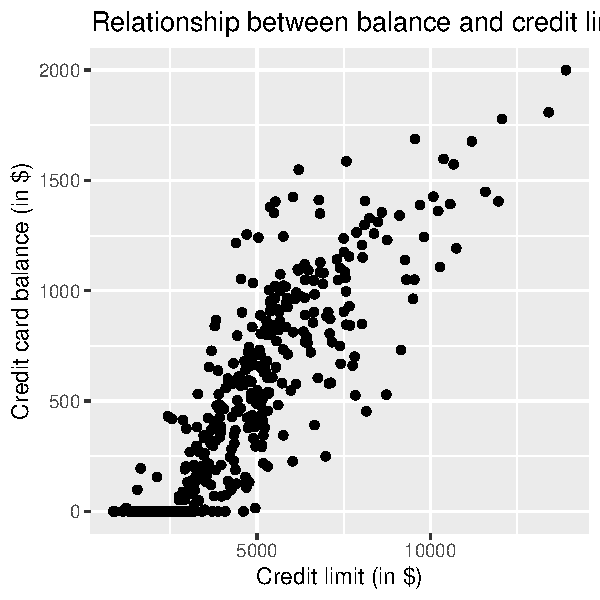
\includegraphics{index_files/figure-pdf/unnamed-chunk-27-1.pdf}

}

\caption{Relationship between balance and credit limit.}

\end{figure}%

Now, let's look at a scatterplot of \texttt{Balance} and
\texttt{Income}:

\begin{Shaded}
\begin{Highlighting}[]
\FunctionTok{ggplot}\NormalTok{(Cred, }\FunctionTok{aes}\NormalTok{(}\AttributeTok{x =}\NormalTok{ Income, }\AttributeTok{y =}\NormalTok{ Balance)) }\SpecialCharTok{+}
  \FunctionTok{geom\_point}\NormalTok{() }\SpecialCharTok{+}
  \FunctionTok{labs}\NormalTok{(}\AttributeTok{x =} \StringTok{"Income (in $1000)"}\NormalTok{, }\AttributeTok{y =} \StringTok{"Credit card balance (in $)"}\NormalTok{, }
       \AttributeTok{title =} \StringTok{"Relationship between balance and income"}\NormalTok{) }
\end{Highlighting}
\end{Shaded}

\begin{figure}[H]

{\centering 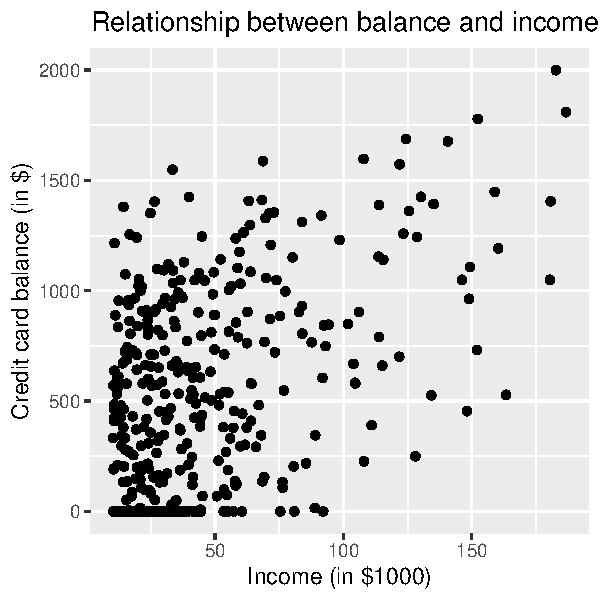
\includegraphics{index_files/figure-pdf/unnamed-chunk-28-1.pdf}

}

\caption{Relationship between balance and income.}

\end{figure}%

The two scatterplots above focus on the relationship between the outcome
variable \texttt{Balance} and each of the explanatory variables
independently. In order to get an idea of the relationship between all
three variables we can use the \texttt{plot\_ly} function within the
\texttt{plotly} library to plot a 3-dimensional scatterplot as follows:

\begin{Shaded}
\begin{Highlighting}[]
\FunctionTok{library}\NormalTok{(plotly)}
\end{Highlighting}
\end{Shaded}

\begin{verbatim}

Attaching package: 'plotly'
\end{verbatim}

\begin{verbatim}
The following object is masked from 'package:ggplot2':

    last_plot
\end{verbatim}

\begin{verbatim}
The following object is masked from 'package:stats':

    filter
\end{verbatim}

\begin{verbatim}
The following object is masked from 'package:graphics':

    layout
\end{verbatim}

\begin{Shaded}
\begin{Highlighting}[]
\FunctionTok{plot\_ly}\NormalTok{(Cred, }\AttributeTok{x =} \SpecialCharTok{\textasciitilde{}}\NormalTok{Income, }\AttributeTok{y =} \SpecialCharTok{\textasciitilde{}}\NormalTok{Limit, }\AttributeTok{z =} \SpecialCharTok{\textasciitilde{}}\NormalTok{Balance,}
        \AttributeTok{type =} \StringTok{"scatter3d"}\NormalTok{, }\AttributeTok{mode =} \StringTok{"markers"}\NormalTok{)}
\end{Highlighting}
\end{Shaded}

\begin{figure}[H]

{\centering 
\includegraphics{index_files/figure-pdf/unnamed-chunk-29-1.pdf}

}

\caption{3D scatterplot of balance, credit limit, and income.}

\end{figure}%

When we fitting our regression model with just a single covariate we
looked at the \emph{best-fitting line}. However, now that we have more
than one explanatory variable, we are looking at the \emph{best-fitting
plane}, which is a 3-dimensional generalisation of the best-fitting
line.

\subsection{Formal analysis}\label{formal-analysis-2}

The multiple regression model we will be fitting to the credit balance
data is given as:

\[y_i = \alpha + \beta_1 x_{1i} + \beta_2 x_{2i} + \epsilon_i, ~~~~ \epsilon \sim N(0, \sigma^2),\]

where

\begin{itemize}
\tightlist
\item
  \(y_i\) is the balance of the \(i^{th}\) individual;
\item
  \(\alpha\) is the intercept and positions the best-fitting plane in 3D
  space;
\item
  \(\beta_1\) is the coefficient for the first explanatory variable
  \(x_1\);
\item
  \(\beta_2\) is the coefficient for the second explanatory variable
  \(x_2\); and
\item
  \(\epsilon_i\) is the \(i^{th}\) random error component.
\end{itemize}

Similarly to a simple linear regression, we use the \texttt{lm} function
to fit the regression model and the \texttt{tab\_model} function to view
our parameter estimates:

\begin{Shaded}
\begin{Highlighting}[]
\NormalTok{Balance.model }\OtherTok{\textless{}{-}} \FunctionTok{lm}\NormalTok{(Balance }\SpecialCharTok{\textasciitilde{}}\NormalTok{ Limit }\SpecialCharTok{+}\NormalTok{ Income, }\AttributeTok{data =}\NormalTok{ Cred)}
\FunctionTok{tab\_model}\NormalTok{(Balance.model,}\AttributeTok{show.ci =}\NormalTok{ F)}
\end{Highlighting}
\end{Shaded}

\begin{longtable}[]{@{}ccc@{}}
\toprule\noalign{}
\endhead
\bottomrule\noalign{}
\endlastfoot
~ & \multicolumn{2}{c@{}}{%
Balance} \\
Predictors & Estimates & p \\
(Intercept) & -385.18 & \textbf{\textless0.001} \\
Limit & 0.26 & \textbf{\textless0.001} \\
Income & -7.66 & \textbf{\textless0.001} \\
Observations & \multicolumn{2}{l@{}}{%
400} \\
R\textsuperscript{2} / R\textsuperscript{2} adjusted &
\multicolumn{2}{l@{}}{%
0.871 / 0.870} \\
\end{longtable}

\begin{tcolorbox}[enhanced jigsaw, leftrule=.75mm, opacityback=0, colbacktitle=quarto-callout-note-color!10!white, left=2mm, rightrule=.15mm, colframe=quarto-callout-note-color-frame, colback=white, coltitle=black, breakable, bottomtitle=1mm, title=\textcolor{quarto-callout-note-color}{\faInfo}\hspace{0.5em}{Note}, toprule=.15mm, titlerule=0mm, toptitle=1mm, bottomrule=.15mm, opacitybacktitle=0.6, arc=.35mm]

To include multiple explanatory variables within a regression model we
simply use the \texttt{+} sign, that is
\texttt{Balance\ \textasciitilde{}\ Limit\ +\ Income}.

\end{tcolorbox}

How do we interpret our model estimates defining the regression plane?
They can be interpreted as follows:

\begin{itemize}
\tightlist
\item
  The \textbf{intercept} represents the credit card balance
  (\texttt{Balance}) of an individual who has \$0 for both credit limit
  (\texttt{Limit}) and income (\texttt{Income}). However, the
  interpretation of the intercept in this case is somewhat limited as
  there are no individuals with \$0 credit limit and income in the data
  set, with the smallest credit card balance being \$0.
\item
  The coefficient for credit limit (\texttt{Limit}) tells us that,
  \emph{taking all other variables in the model into account}, that
  there is an associated increase, on average, in credit card balance of
  \$0.26.
\item
  Similarly, the coefficient for income (\texttt{Income}) tells us that,
  \emph{taking all other variables in the model into account}, that
  there is an associated decrease, on average, in credit card balance of
  \$7.66.
\end{itemize}

What do you notice that is strange about our coefficient estimates given
our exploratory data analysis? Well, from our scatterplots of credit
card balance against both credit limit and income, we seen that there
appeared to be a positive linear relationship. Then, why do we then get
a negative coefficient for income (-7.66)? This is due to a phenomenon
known as \textbf{Simpson's Paradox}. This occurs when there are trends
within different categories (or groups) of data, but that these trends
disappear when the categories are grouped as a whole. For more details
see
\href{https://moderndive.com/6-multiple-regression.html\#simpsonsparadox}{Section
6.3.4 of An Introduction to Statistical and Data Sciences in R}.

\subsection{Assessing model fit for multiple
regression}\label{assessing-model-fit-for-multiple-regression}

Now we need to assess our model assumptions. Similarly to simple
regression, our model assumptions are:

\begin{enumerate}
\def\labelenumi{\arabic{enumi}.}
\tightlist
\item
  The deterministic part of the model captures all the non-random
  structure in the data, i.e.~the residuals have mean zero.
\item
  The scale of the variability of the residuals is constant at all
  values of the explanatory variables.
\item
  The residuals are normally distributed.
\item
  The residuals are independent.
\item
  The values of the explanatory variables are recorded without error.
\end{enumerate}

First, we need to obtain the fitted values and residuals from our
regression model:

\begin{Shaded}
\begin{Highlighting}[]
\NormalTok{Balance.model\_output }\OtherTok{\textless{}{-}}\NormalTok{  Cred }\SpecialCharTok{\%\textgreater{}\%} 
  \FunctionTok{mutate}\NormalTok{(}\AttributeTok{Balance\_hat  =}\NormalTok{ Balance.model}\SpecialCharTok{$}\NormalTok{fitted.values,}
         \AttributeTok{residual =}\NormalTok{ Balance.model}\SpecialCharTok{$}\NormalTok{residuals)}
\end{Highlighting}
\end{Shaded}

We can assess our first two model assumptions by producing scatterplots
of our residuals against each of our explanatory variables. First, let's
begin with the scatterplot of the residuals against credit limit:

\begin{Shaded}
\begin{Highlighting}[]
\FunctionTok{ggplot}\NormalTok{(Balance.model\_output, }\FunctionTok{aes}\NormalTok{(}\AttributeTok{x =}\NormalTok{ Limit, }\AttributeTok{y =}\NormalTok{ residual)) }\SpecialCharTok{+}
  \FunctionTok{geom\_point}\NormalTok{() }\SpecialCharTok{+}
  \FunctionTok{labs}\NormalTok{(}\AttributeTok{x =} \StringTok{"Credit limit (in $)"}\NormalTok{, }\AttributeTok{y =} \StringTok{"Residual"}\NormalTok{, }\AttributeTok{title =} \StringTok{"Residuals vs credit limit"}\NormalTok{)  }\SpecialCharTok{+}
  \FunctionTok{geom\_hline}\NormalTok{(}\AttributeTok{yintercept =} \DecValTok{0}\NormalTok{, }\AttributeTok{col =} \StringTok{"blue"}\NormalTok{, }\AttributeTok{linewidth =} \DecValTok{1}\NormalTok{)}
\end{Highlighting}
\end{Shaded}

\begin{figure}[H]

{\centering 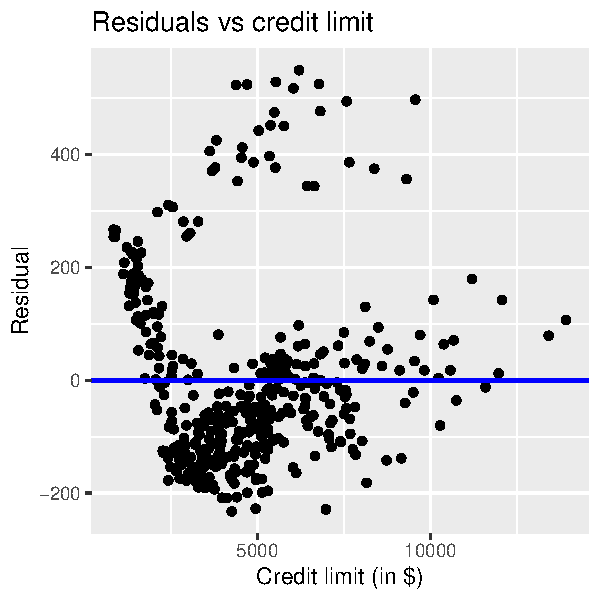
\includegraphics{index_files/figure-pdf/unnamed-chunk-31-1.pdf}

}

\caption{Residuals vs credit limit.}

\end{figure}%

Now, let's plot a scatterplot of the residuals against income:

\begin{Shaded}
\begin{Highlighting}[]
\FunctionTok{ggplot}\NormalTok{(Balance.model\_output, }\FunctionTok{aes}\NormalTok{(}\AttributeTok{x =}\NormalTok{ Income, }\AttributeTok{y =}\NormalTok{ residual)) }\SpecialCharTok{+}
  \FunctionTok{geom\_point}\NormalTok{() }\SpecialCharTok{+}
  \FunctionTok{labs}\NormalTok{(}\AttributeTok{x =} \StringTok{"Income (in $1000)"}\NormalTok{, }\AttributeTok{y =} \StringTok{"Residual"}\NormalTok{, }\AttributeTok{title =} \StringTok{"Residuals vs income"}\NormalTok{) }\SpecialCharTok{+}
  \FunctionTok{geom\_hline}\NormalTok{(}\AttributeTok{yintercept =} \DecValTok{0}\NormalTok{, }\AttributeTok{col =} \StringTok{"blue"}\NormalTok{, }\AttributeTok{linewidth =} \DecValTok{1}\NormalTok{)}
\end{Highlighting}
\end{Shaded}

\begin{figure}[H]

{\centering 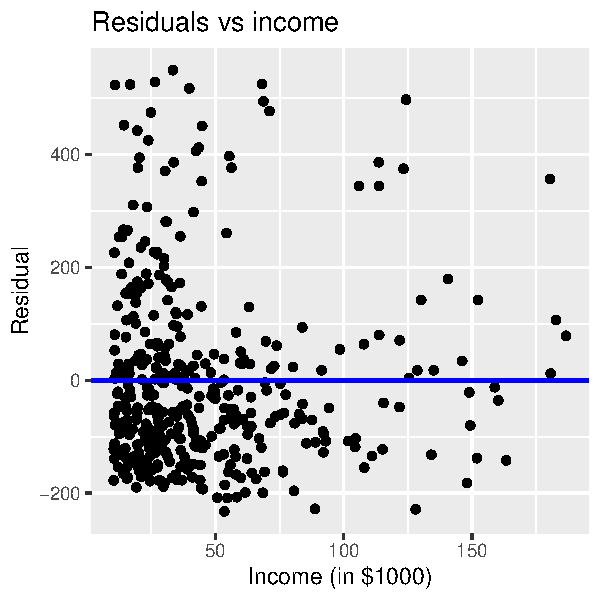
\includegraphics{index_files/figure-pdf/unnamed-chunk-32-1.pdf}

}

\caption{Residuals vs income.}

\end{figure}%

Alternatively, we can use the \texttt{check\_model} function to produce
the standard diagnostic plots for a fitted linear regression model:

\begin{Shaded}
\begin{Highlighting}[]
\FunctionTok{check\_model}\NormalTok{(Balance.model, }\AttributeTok{check=} \FunctionTok{c}\NormalTok{(}\StringTok{"linearity"}\NormalTok{,}\StringTok{"homogeneity"}\NormalTok{,}\StringTok{"qq"}\NormalTok{,}\StringTok{"normality"}\NormalTok{))}
\end{Highlighting}
\end{Shaded}

\begin{figure}[H]

{\centering 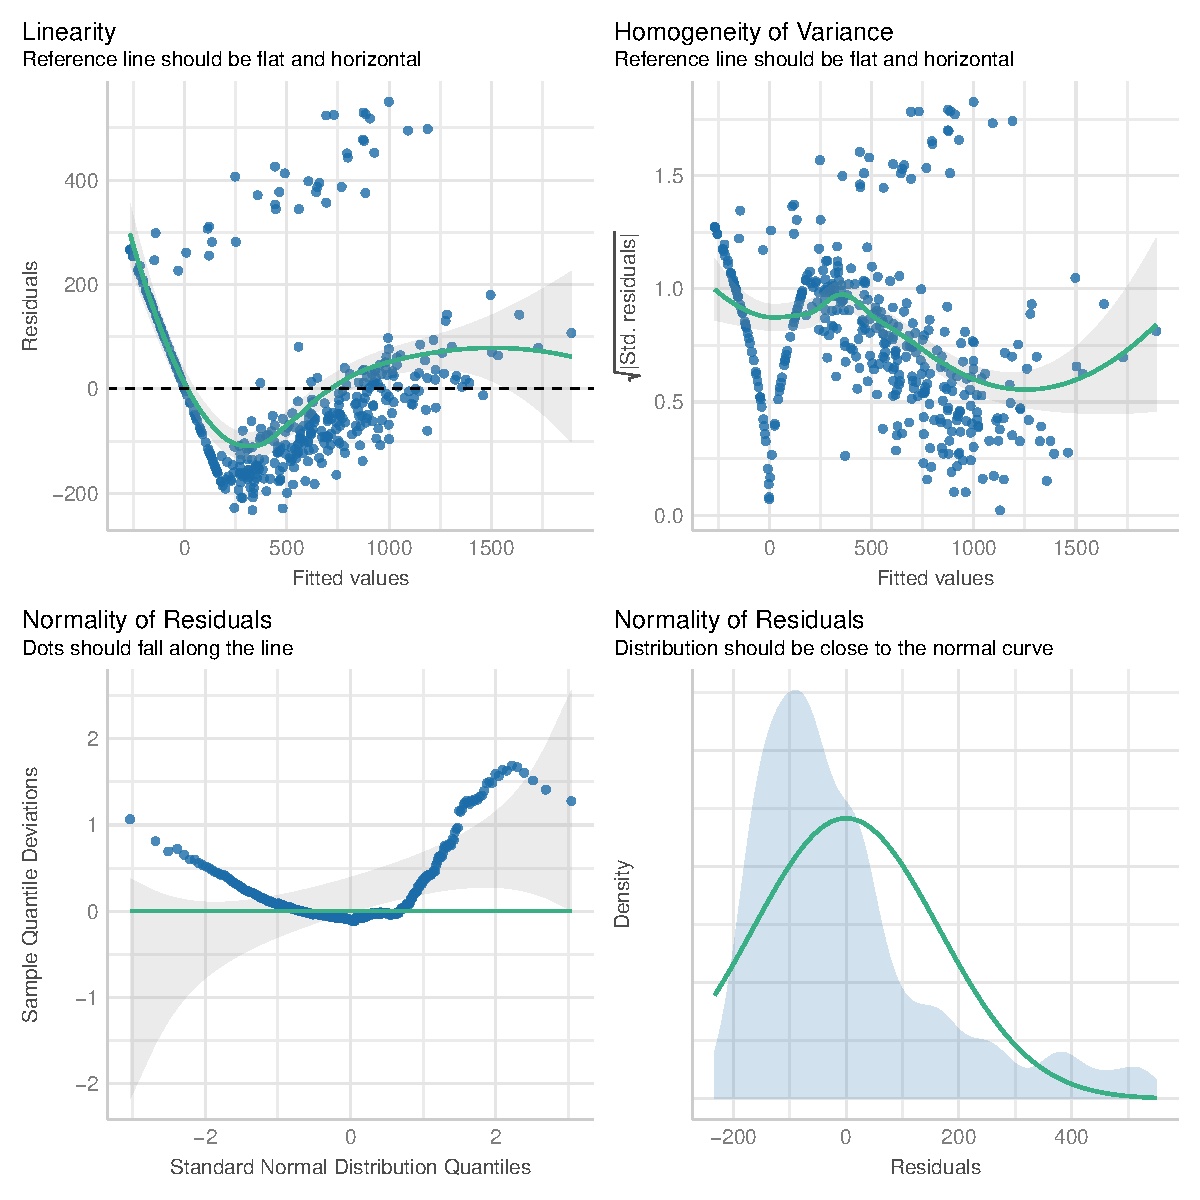
\includegraphics{index_files/figure-pdf/unnamed-chunk-33-1.pdf}

}

\caption{Balance.model Residuals checks.}

\end{figure}%

\begin{tcolorbox}[enhanced jigsaw, leftrule=.75mm, opacityback=0, colbacktitle=quarto-callout-tip-color!10!white, left=2mm, rightrule=.15mm, colframe=quarto-callout-tip-color-frame, colback=white, coltitle=black, breakable, bottomtitle=1mm, title={Question}, toprule=.15mm, titlerule=0mm, toptitle=1mm, bottomrule=.15mm, opacitybacktitle=0.6, arc=.35mm]

Which assumptions does each of the following plots address?

\end{tcolorbox}

\begin{tcolorbox}[enhanced jigsaw, leftrule=.75mm, opacityback=0, colbacktitle=quarto-callout-warning-color!10!white, left=2mm, rightrule=.15mm, colframe=quarto-callout-warning-color-frame, colback=white, coltitle=black, breakable, bottomtitle=1mm, title={Task}, toprule=.15mm, titlerule=0mm, toptitle=1mm, bottomrule=.15mm, opacitybacktitle=0.6, arc=.35mm]

Use the \texttt{plot\_model} function from the \texttt{sjPlot} package
to obtain the same diagnostic plots produced via
\texttt{check\_model(Balance.model,\ check=\ c(homogeneity","qq","normality"))}.

Click here to see the solution

\begin{Shaded}
\begin{Highlighting}[]
\NormalTok{diag\_plots }\OtherTok{=} \FunctionTok{plot\_model}\NormalTok{(Balance.model,}\AttributeTok{type=}\StringTok{\textquotesingle{}diag\textquotesingle{}}\NormalTok{)}

\CommentTok{\# QQ plot}
\NormalTok{diag\_plots[[}\DecValTok{2}\NormalTok{]]}
\end{Highlighting}
\end{Shaded}

\begin{verbatim}
`geom_smooth()` using formula = 'y ~ x'
\end{verbatim}

\begin{center}
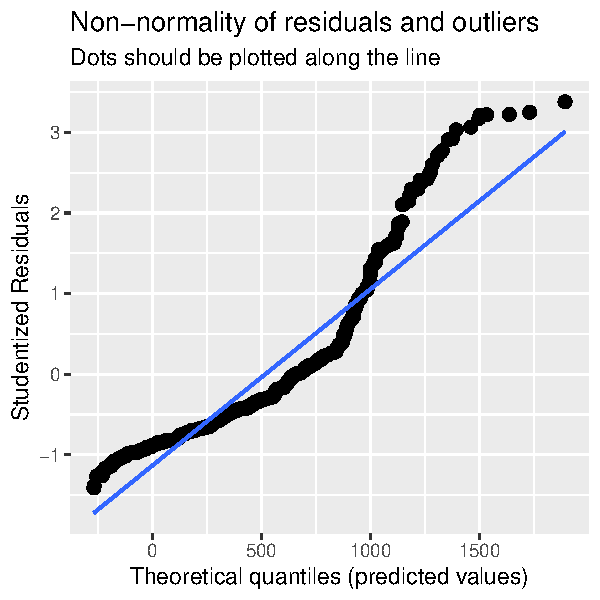
\includegraphics{index_files/figure-pdf/unnamed-chunk-34-1.pdf}
\end{center}

\begin{Shaded}
\begin{Highlighting}[]
\CommentTok{\# Histrogram/density plot}
\NormalTok{diag\_plots[[}\DecValTok{3}\NormalTok{]]}
\end{Highlighting}
\end{Shaded}

\begin{center}
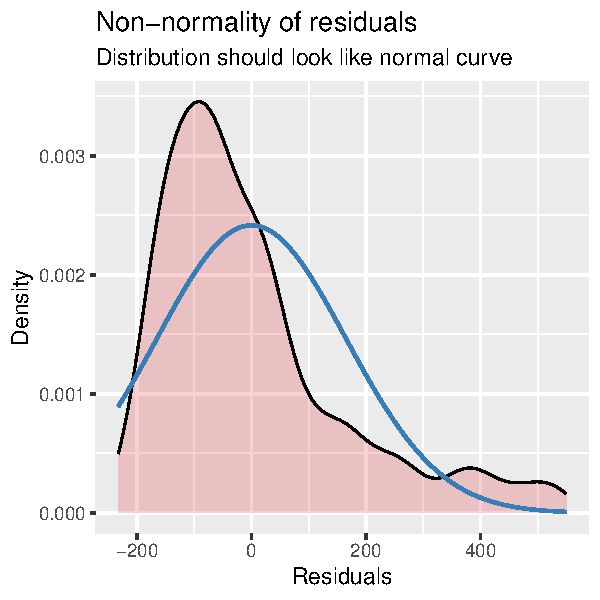
\includegraphics{index_files/figure-pdf/unnamed-chunk-34-2.pdf}
\end{center}

\begin{Shaded}
\begin{Highlighting}[]
\CommentTok{\# Residuals vs fitted values}
\NormalTok{diag\_plots[[}\DecValTok{4}\NormalTok{]]}
\end{Highlighting}
\end{Shaded}

\begin{verbatim}
`geom_smooth()` using formula = 'y ~ x'
\end{verbatim}

\begin{center}
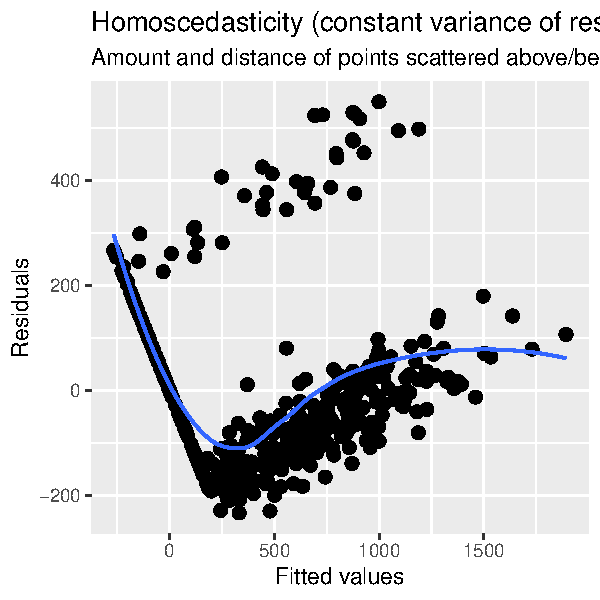
\includegraphics{index_files/figure-pdf/unnamed-chunk-34-3.pdf}
\end{center}

\end{tcolorbox}

Lastly, besides our usual diagnostic plots to checks we need to be
carefull with the collinearity among our predictor since a high
collinearity value may inflate the parameter uncertainty.

To check for colliniearity we can compute the VIF (Variance Inflation
Factor) which measures how well a covariate \(j\) can be predicted by
all other predictors in the model. It measures how much the variance of
a regression coefficient is inflated due to collinearity.

It is computed by regressing a predicor \(x_j\) against all other
predictors in the model and then obtaining the VIF as:

\[
VIF_j = \frac{1}{1-R^2_j}
\] where \(R^2_j\) is the coefficient of determination from this
auxiliary regression. In general terms we can interpret VIF as follows:

\begin{itemize}
\item
  VIF = 1: No multicollinearity (predictor is uncorrelated with others).
\item
  1 \(<\) VIF \textless{} 5: Moderate correlation (usually acceptable).
\item
  VIF \(\geq\) 5: High multicollinearity (may inflate coefficient
  variance, reducing reliability).
\end{itemize}

We can check for collinearity using the \texttt{check\_model} function
as follows:

\begin{Shaded}
\begin{Highlighting}[]
\FunctionTok{check\_model}\NormalTok{(Balance.model,}\AttributeTok{check=}\StringTok{"vif"}\NormalTok{)}
\end{Highlighting}
\end{Shaded}

\begin{center}
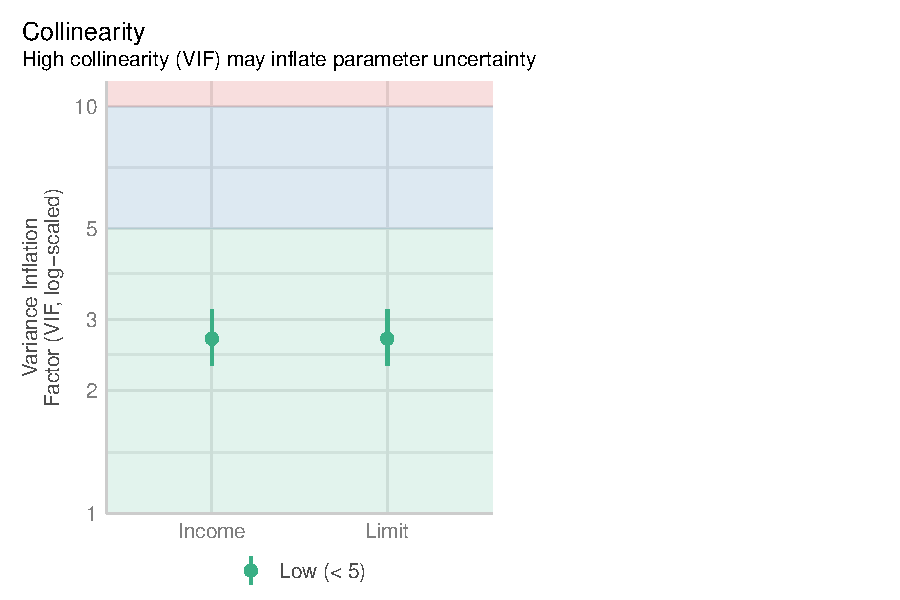
\includegraphics{index_files/figure-pdf/unnamed-chunk-35-1.pdf}
\end{center}

Alternatively, the aforementioned \texttt{plot\_model()} function from
\texttt{sjPlot} also compute this as part of the default diagnostic
plots:

\begin{Shaded}
\begin{Highlighting}[]
\NormalTok{diag\_plots[[}\DecValTok{1}\NormalTok{]]}
\end{Highlighting}
\end{Shaded}

\begin{center}
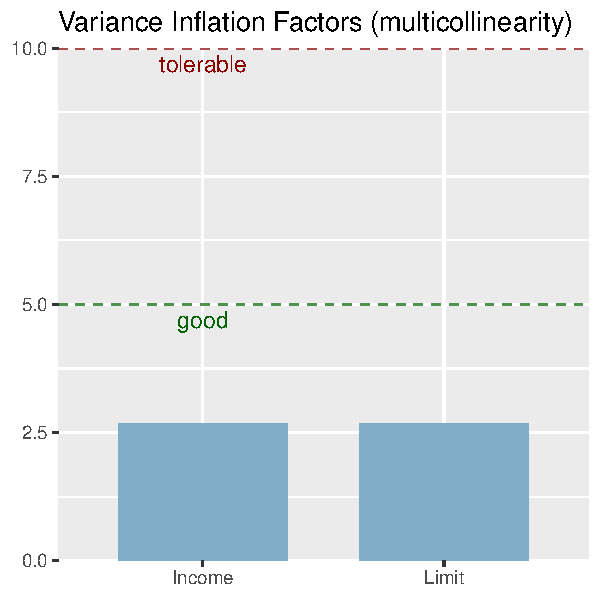
\includegraphics{index_files/figure-pdf/unnamed-chunk-36-1.pdf}
\end{center}

You can further enhance your data analysis skills by completing the
additional \href{about.qmd}{tasks}. Attempt these tasks first, then
compare your solutions with the provided answers.



\end{document}
